% Options for packages loaded elsewhere
\PassOptionsToPackage{unicode}{hyperref}
\PassOptionsToPackage{hyphens}{url}
\PassOptionsToPackage{dvipsnames,svgnames,x11names}{xcolor}
%
\documentclass[
  number,
  3p]{elsarticle}

\usepackage{amsmath,amssymb}
\usepackage{lmodern}
\usepackage{iftex}
\ifPDFTeX
  \usepackage[T1]{fontenc}
  \usepackage[utf8]{inputenc}
  \usepackage{textcomp} % provide euro and other symbols
\else % if luatex or xetex
  \usepackage{unicode-math}
  \defaultfontfeatures{Scale=MatchLowercase}
  \defaultfontfeatures[\rmfamily]{Ligatures=TeX,Scale=1}
\fi
% Use upquote if available, for straight quotes in verbatim environments
\IfFileExists{upquote.sty}{\usepackage{upquote}}{}
\IfFileExists{microtype.sty}{% use microtype if available
  \usepackage[]{microtype}
  \UseMicrotypeSet[protrusion]{basicmath} % disable protrusion for tt fonts
}{}
\makeatletter
\@ifundefined{KOMAClassName}{% if non-KOMA class
  \IfFileExists{parskip.sty}{%
    \usepackage{parskip}
  }{% else
    \setlength{\parindent}{0pt}
    \setlength{\parskip}{6pt plus 2pt minus 1pt}}
}{% if KOMA class
  \KOMAoptions{parskip=half}}
\makeatother
\usepackage{xcolor}
\setlength{\emergencystretch}{3em} % prevent overfull lines
\setcounter{secnumdepth}{-\maxdimen} % remove section numbering
% Make \paragraph and \subparagraph free-standing
\ifx\paragraph\undefined\else
  \let\oldparagraph\paragraph
  \renewcommand{\paragraph}[1]{\oldparagraph{#1}\mbox{}}
\fi
\ifx\subparagraph\undefined\else
  \let\oldsubparagraph\subparagraph
  \renewcommand{\subparagraph}[1]{\oldsubparagraph{#1}\mbox{}}
\fi


\providecommand{\tightlist}{%
  \setlength{\itemsep}{0pt}\setlength{\parskip}{0pt}}\usepackage{longtable,booktabs,array}
\usepackage{calc} % for calculating minipage widths
% Correct order of tables after \paragraph or \subparagraph
\usepackage{etoolbox}
\makeatletter
\patchcmd\longtable{\par}{\if@noskipsec\mbox{}\fi\par}{}{}
\makeatother
% Allow footnotes in longtable head/foot
\IfFileExists{footnotehyper.sty}{\usepackage{footnotehyper}}{\usepackage{footnote}}
\makesavenoteenv{longtable}
\usepackage{graphicx}
\makeatletter
\def\maxwidth{\ifdim\Gin@nat@width>\linewidth\linewidth\else\Gin@nat@width\fi}
\def\maxheight{\ifdim\Gin@nat@height>\textheight\textheight\else\Gin@nat@height\fi}
\makeatother
% Scale images if necessary, so that they will not overflow the page
% margins by default, and it is still possible to overwrite the defaults
% using explicit options in \includegraphics[width, height, ...]{}
\setkeys{Gin}{width=\maxwidth,height=\maxheight,keepaspectratio}
% Set default figure placement to htbp
\makeatletter
\def\fps@figure{htbp}
\makeatother
\newlength{\cslhangindent}
\setlength{\cslhangindent}{1.5em}
\newlength{\csllabelwidth}
\setlength{\csllabelwidth}{3em}
\newlength{\cslentryspacingunit} % times entry-spacing
\setlength{\cslentryspacingunit}{\parskip}
\newenvironment{CSLReferences}[2] % #1 hanging-ident, #2 entry spacing
 {% don't indent paragraphs
  \setlength{\parindent}{0pt}
  % turn on hanging indent if param 1 is 1
  \ifodd #1
  \let\oldpar\par
  \def\par{\hangindent=\cslhangindent\oldpar}
  \fi
  % set entry spacing
  \setlength{\parskip}{#2\cslentryspacingunit}
 }%
 {}
\usepackage{calc}
\newcommand{\CSLBlock}[1]{#1\hfill\break}
\newcommand{\CSLLeftMargin}[1]{\parbox[t]{\csllabelwidth}{#1}}
\newcommand{\CSLRightInline}[1]{\parbox[t]{\linewidth - \csllabelwidth}{#1}\break}
\newcommand{\CSLIndent}[1]{\hspace{\cslhangindent}#1}

% Energy commands
\newcommand{\E}[2][]{E^{\mathrm{#1}}_{\mathrm{#2}}}
\newcommand{\DeltaE}[2][]{\Delta E^{\mathrm{#1}}_{\mathrm{#2}}}
\newcommand{\DeltaEST}[2][]{\Delta E^{\mathrm{#1}}_{\mathrm{ST,#2}}}
\newcommand{\EState}[2][]{E (\phi_{\mathrm{#2}}^{#1})}

% Integrals
\newcommand{\Integral}[1]{(i | K_x #1 K_y | k )^2}
\makeatletter
\makeatother
\makeatletter
\makeatother
\makeatletter
\@ifpackageloaded{caption}{}{\usepackage{caption}}
\AtBeginDocument{%
\ifdefined\contentsname
  \renewcommand*\contentsname{Table of contents}
\else
  \newcommand\contentsname{Table of contents}
\fi
\ifdefined\listfigurename
  \renewcommand*\listfigurename{List of Figures}
\else
  \newcommand\listfigurename{List of Figures}
\fi
\ifdefined\listtablename
  \renewcommand*\listtablename{List of Tables}
\else
  \newcommand\listtablename{List of Tables}
\fi
\ifdefined\figurename
  \renewcommand*\figurename{Figure}
\else
  \newcommand\figurename{Figure}
\fi
\ifdefined\tablename
  \renewcommand*\tablename{Table}
\else
  \newcommand\tablename{Table}
\fi
}
\@ifpackageloaded{float}{}{\usepackage{float}}
\floatstyle{ruled}
\@ifundefined{c@chapter}{\newfloat{codelisting}{h}{lop}}{\newfloat{codelisting}{h}{lop}[chapter]}
\floatname{codelisting}{Listing}
\newcommand*\listoflistings{\listof{codelisting}{List of Listings}}
\makeatother
\makeatletter
\@ifpackageloaded{caption}{}{\usepackage{caption}}
\@ifpackageloaded{subcaption}{}{\usepackage{subcaption}}
\makeatother
\makeatletter
\@ifpackageloaded{tcolorbox}{}{\usepackage[many]{tcolorbox}}
\makeatother
\makeatletter
\@ifundefined{shadecolor}{\definecolor{shadecolor}{rgb}{.97, .97, .97}}
\makeatother
\makeatletter
\makeatother
\journal{Journal of Physical Chemistry A}
\ifLuaTeX
  \usepackage{selnolig}  % disable illegal ligatures
\fi
\IfFileExists{bookmark.sty}{\usepackage{bookmark}}{\usepackage{hyperref}}
\IfFileExists{xurl.sty}{\usepackage{xurl}}{} % add URL line breaks if available
\urlstyle{same} % disable monospaced font for URLs
\hypersetup{
  pdftitle={Ultrafast computational screening of molecules with inverted singlet-triplet energy gaps using semi-empirical quantum chemistry},
  pdfauthor={Kjell Jorner; Robert Pollice; Cyrille Lavigne; Alán Aspuru Guzik},
  colorlinks=true,
  linkcolor={blue},
  filecolor={Maroon},
  citecolor={Blue},
  urlcolor={Blue},
  pdfcreator={LaTeX via pandoc}}

\setlength{\parindent}{6pt}
\begin{document}

\begin{frontmatter}
\title{Ultrafast computational screening of molecules with inverted
singlet-triplet energy gaps using semi-empirical quantum chemistry}
\author[1,2,3,4]{Kjell Jorner%
\corref{cor1}%
}
 \ead{kjell.jorner@chem.ethz.ch} 
\author[5,3,4]{Robert Pollice%
\corref{cor1}%
}
 \ead{r.pollice@rug.nl} 
\author[3,4]{Cyrille Lavigne%
%
}

\author[3,4,6,7,8,10]{Alán Aspuru Guzik%
%
}


\affiliation[1]{organization={ETH Zürich, Institute of Chemical and
Bioengineering, Department of Chemistry and Applied
Biosciences},addressline={Vladimir-Prelog-Weg
1},city={Zürich},country={Switzerland},countrysep={,},postcode={CH-8093},postcodesep={}}
\affiliation[2]{organization={Chalmers University of
Technology, Department of Chemistry and Chemical
Engineering},addressline={Kemigården
4},city={Gothenburg},country={Sweden},countrysep={,},postcode={SE-41258},postcodesep={}}
\affiliation[3]{organization={University of Toronto, Chemical Physics
Theory Group, Department of Chemistry},addressline={80 St.~George
St.},city={Toronto},country={Canada},countrysep={,},postcode={M5S
3H6},postcodesep={}}
\affiliation[4]{organization={University of Toronto, Department of
Computer Science},addressline={40 St.~George
St.},city={Toronto},country={Canada},countrysep={,},postcode={M5S
2E4},postcodesep={}}
\affiliation[5]{organization={University of Groningen, Stratingh
Institute for Chemistry},addressline={Nijenborgh
4},city={Groningen},country={The
Netherlands},countrysep={,},postcode={9747 AG},postcodesep={}}
\affiliation[6]{organization={University of Toronto, Department of
Chemical Engineering \& Applied Chemistry},addressline={200 College
St.},city={Toronto},country={Canada},countrysep={,},postcode={M5S
3E5},postcodesep={}}
\affiliation[7]{organization={University of Toronto, Department of
Materials Science \& Engineering},addressline={184 College
St.},city={Toronto},country={Canada},countrysep={,},postcode={M5S
3E4},postcodesep={}}
\affiliation[8]{organization={Vector Institute for Artificial
Intelligence},addressline={661 University Ave. Suite
710},city={Toronto},country={Canada},countrysep={,},postcode={M5G
1M1},postcodesep={}}
\affiliation[9]{organization={Lebovic Fellow, Canadian Institute for
Advanced Research
(CIFAR)},city={Toronto},country={Canada},countrysep={,},postcode={M5G
1M1},postcodesep={}}
\affiliation[10]{organization={Acceleration Consortium, University of
Toronto},city={Toronto},country={Canada},countrysep={,},postcodesep={}}

\cortext[cor1]{Corresponding author}




        
\begin{abstract}
Molecules with an inverted energy gap between their first excited states
of singlet and triplet multiplicity have promising applications in the
next generation of organic light-emitting diode (OLED) materials.
Unfortunately, such molecules are rare and only a handful of examples
are currently known. High-throughput virtual screening could assist in
finding novel classes of molecules, but current efforts are hampered by
the high computational cost of the required quantum-chemical methods. We
present a method based on the semi-empirical Pariser-Parr-Pople theory
augmented by perturbation theory and show that it reproduces inverted
gaps at a fraction of the cost of the current employed methods. Our
study opens the doors for ultra-high-throughput virtual screening and
inverse design to accelerate the discovery and development of the new
generation of OLED materials.
\end{abstract}





\end{frontmatter}
    \ifdefined\Shaded\renewenvironment{Shaded}{\begin{tcolorbox}[breakable, interior hidden, frame hidden, sharp corners, boxrule=0pt, enhanced, borderline west={3pt}{0pt}{shadecolor}]}{\end{tcolorbox}}\fi

\hypertarget{introduction}{%
\section{Introduction}\label{introduction}}

Organic light-emitting diodes (OLEDs) is a technology for generating
light from electricity using organic
molecules.\textsuperscript{\protect\hyperlink{ref-yangRecentAdvancesOrganic2017}{1}}
The first generation of OLEDs were limited to an efficiency of max 25\%
due to spin statistics. As the transition T\textsubscript{1}
\(\rightarrow\) S\textsubscript{0}, from the lowest excited triplet
state to the singlet ground state, is quantum-mechanically forbidden,
the OLED molecule can formally only emit from its first excited state of
singlet multiplicity, S\textsubscript{1}. The second generation of OLEDs
exploited ways of increasing the rate of this spin-forbidden
phosphorescence. The third generation of OLEDs are based on Thermally
Activated Delayed Fluorescence (TADF), where the S\textsubscript{1}
state is partially populated from a near-lying T\textsubscript{1} state.
For this to happen, the gap \(\DeltaE{ST}\) between the states needs to
sufficiently small so that the thermal activation competes with
non-radiative decay processes from T\textsubscript{1}. However, as the
T\textsubscript{1} population is still substantial, problems with
stability and lower than ideal intensity due to non-radiative decay
persist. The logical step for the next generation of OLEDs is to emit
directly from an S\textsubscript{1} state that lies below the
T\textsubscript{1} state, potentially converting all of the electrically
generated excitons into photons, \emph{i.e.}, 100\% efficiency.

Molecules that fulfill this criterion have been branded with the acronym
INVErted Singlet Triplet energy gap (INVEST) and are exceedingly
rare.\textsuperscript{\protect\hyperlink{ref-liOrganicMoleculesInverted2022}{2}}
They are said to violate Hund's rule of maximum multiplicity, which
describes that the electronic state with the highest spin (in this case
the triplet) should be lowest in energy. While examples of molecules
violating Hund's rule in the excited state have been known since the
1970s and
1980s,\textsuperscript{\protect\hyperlink{ref-kollmarViolationHundRule1978}{3}--\protect\hyperlink{ref-kosekiViolationHundMultiplicity1985}{5}}
it is only recently that they have received considerable attention for
application in
OLEDs.\textsuperscript{\protect\hyperlink{ref-desilvaInvertedSingletTriplet2019}{6}--\protect\hyperlink{ref-aizawaDelayedFluorescenceInverted2022}{8}}
As they are rare, recent efforts have used high-throughput virtual
screening (HTVS) with computational chemistry to identify new compounds
with inverted gaps, focusing on expanding the local chemical space
around specific
scaffolds\textsuperscript{\protect\hyperlink{ref-polliceOrganicMoleculesInverted2021}{7},\protect\hyperlink{ref-aizawaDelayedFluorescenceInverted2022}{8}}
or scanning larger (combinatorially or experimentally derived) datasets
to identify novel
scaffolds.\textsuperscript{\protect\hyperlink{ref-terenceblaskovitsSymmetryInducedSinglet2023}{9}--\protect\hyperlink{ref-garnerDoublebondDelocalizationNonalternant2023}{11}}
These HTVS efforts have been successful at identifying several new
INVEST candidates, some of which have also been synthesized and tested
experimentally.\textsuperscript{\protect\hyperlink{ref-aizawaDelayedFluorescenceInverted2022}{8}}

While this early success of HTVS is highly encouraging, it is hampered
by the cost of the computational methods. Excitation energies are
routinely calculated by time-dependent density functional theory
(TD-DFT), which has become a workhorse of computational photophysics
over the last
decades.\textsuperscript{\protect\hyperlink{ref-casidaProgressTimeDependentDensityFunctional2012}{12}}
Unfortunately, it has been shown that TD-DFT fails to capture the
inverted gap of INVEST compounds, as the method only considers single
electronic
excitations.\textsuperscript{\protect\hyperlink{ref-desilvaInvertedSingletTriplet2019}{6}}
Inclusion of at least double excitations are necessary to reproduce the
inverted gaps, corresponding to methods such as double hybrid TD-DFT or
excited state coupled-cluster methods such as second-order approximate
coupled cluster singles and doubles (CC2) or equation of motion coupled
cluster with single and double excitations (EOM-CCSD). In line with the
results of benchmarking
studies,\textsuperscript{\protect\hyperlink{ref-ricciSingletTripletExcited2021}{13},\protect\hyperlink{ref-sancho-garciaViolationHundRule2022}{14}}
recent HTVS studies have used methods such as the complete active space
self-consistent field (CASSCF) and CC2 for preliminary screening, while
confirming inverted gaps with more expensive methods such as multistate
complete active space second-order perturbation theory (MS-CASPT2) and
EOM-CCSD. These methods are not only expensive, but in the case of the
CAS methods, also require the choice of an orbital active space,
something which is not routinely automatized.

Motivated by the need for faster methods for HTVS of INVEST compounds,
we wondered if it would be possible to perform much simpler calculations
as a pre-screening step for the more expensive methods. Based on prior
work in the literature from the 1970s and 1980s, we find that the
inverted gaps can be recovered already with the semi-empirical
Pariser-Parr-Pople method using configuration interaction singles (CIS)
and adding key double excitations. The PPP method considers only the
\(\pi\) electrons in a minimal valence basis and approximates all
integrals from experimental data and a few empirical parameters, making
it computationally extremely cheap. At the same time, it retains the
conceptual clarity of Hückel theory and allows for straightforward
interpretation of the inverted gap in terms of the well-known concept of
dynamic spin polarization (DSP). We show that the method is capable of
finding hits both in the local chemical space around known scaffolds,
and of identifying hits in more diverse datasets. While there are clear
limitations to the method, we believe that it will open the doors for
ultra high-throughput virtual screening (UHTVS) of compound libraries
orders of magnitude larger than today. The method is also perfectly
applicable as a scoring function in inverse design algorithms.

\hypertarget{theory}{%
\section{Theory}\label{theory}}

While the recent literature has focused on applying high-level \emph{ab
initio} and DFT methods to study INVEST compounds, we believe that some
conceptual clarity has been lost in process. Instead, we apply the
simplest possible electronic structure method that can capture the
physics of the problem. The Pariser-Parr-Pople (PPP) method is an
extension of the semi-empirical Hückel molecular orbital theory for
\(\pi\)-electron systems that includes electron
correlation.\textsuperscript{\protect\hyperlink{ref-pariserSemiEmpiricalTheory1953a}{15}--\protect\hyperlink{ref-popleElectronInteractionUnsaturated1953}{17}}
It originated in the 1950s, with new parametrizations being developed
mainly in the 1960s and 1970s, and was used in the dye industry at least
until the 1980s before the advent of more accurate ab initio
methods.\textsuperscript{\protect\hyperlink{ref-griffithsPracticalAspectsColour1982}{18}}
The PPP method retains the conceptual clarity of Hückel theory, while at
the same time including the electron correlation that is necessary to
capture the inverted gap.

\hypertarget{pariser-parr-pople-theory}{%
\subsection{Pariser-Parr-Pople theory}\label{pariser-parr-pople-theory}}

Within Pople's formulation of PPP theory, Roothan's equations are solved
self-consistently.\textsuperscript{\protect\hyperlink{ref-popleElectronInteractionUnsaturated1953}{17}}.
Under the Zero Differential Overlap (ZDO) approximation, overlap
integrals are neglected for orbitals on different centers, leading to a
simplification of the Roothan equations as \(\mathbf{S}\) becomes the
unit matrix \(\mathbf{I}\)

\begin{equation}\protect\hypertarget{eq-roothan}{}{
\mathbf{FC} = \mathbf{SCE} = \mathbf{ICE} = \mathbf{CE}
}\label{eq-roothan}\end{equation}

where \(\mathbf{F}\) is the Fock matrix, \(\mathbf{C}\) contains the
molecular orbital coefficients and \(\mathbf{E}\) is the diagonal matrix
of the orbital energy eigenvalues. Given \(\mathbf{F}\), the
corresponding \(\mathbf{C}\) and \(\mathbf{E}\) can then be determined
either self-consistently (following
Pople\textsuperscript{\protect\hyperlink{ref-popleElectronInteractionUnsaturated1953}{17}})
or via configuration interaction (following Pariser and
Parr\textsuperscript{\protect\hyperlink{ref-pariserSemiEmpiricalTheory1953a}{15},\protect\hyperlink{ref-pariserSemiEmpiricalTheory1953}{16}}),
most often starting from a guess \(\mathbf{C}\) from the corresponding
Hückel model. The main effort is then to construct \(\mathbf{F}\), which
has the following matrix
elements\textsuperscript{\protect\hyperlink{ref-beveridgeParametrizationSemiempiricalPi1971}{19}}
\begin{equation}\protect\hypertarget{eq-f-rr}{}{
F_{rr} = H_{rr} + \sum_{t} P_{tt} \gamma_{rt} - \frac{1}{2} P_{rr} \gamma_{rr} 
}\label{eq-f-rr}\end{equation}

\begin{equation}\protect\hypertarget{eq-f-rs}{}{
F_{rs} = H_{rs} - \frac{1}{2} P_{rs} \gamma_{rs}
}\label{eq-f-rs}\end{equation}

where \(P_{rs}\) are elements of the density matrix \(\mathbf{P}\) and
\(\gamma_{rr}\) and \(\gamma_{rs}\) are parameters called the
\emph{one-center and two-center electron repulsion integrals},
respectively. The \emph{core resonance integral} matrix elements of
\(\mathbf{H}\) are given by
\begin{equation}\protect\hypertarget{eq-h-rr}{}{
H_{rr} = \alpha_r = U_r - \sum_{s \neq r} Z_s \gamma_{rs}
}\label{eq-h-rr}\end{equation}
\begin{equation}\protect\hypertarget{eq-h-rs}{}{
H_{rs} = \beta_{rs}
}\label{eq-h-rs}\end{equation}

where \(\alpha_{r}\) is the \emph{one-center core resonance integral},
\(U_r\) is a parameter of model called the \emph{atomic valence state
potential}, \(Z_s\) is the effective nuclear charge and \(\beta_{rs}\)
is the \emph{two-center resonance integral}, another parameter of the
model.

\hypertarget{parametrization}{%
\subsection{Parametrization}\label{parametrization}}

The four parameters are thus \(U_{r}\), \(\gamma_{rr}\), \(\gamma_{rs}\)
and \(\beta_{rs}\). They are derived either from experiment, first
principles, or a combination of both. The Pariser-Parr approximation
leads to \begin{equation}\protect\hypertarget{eq-u-r}{}{
U_{r} = - \mathrm{IP}_v
}\label{eq-u-r}\end{equation}

where \(\mathrm{IP}_v\) is the \emph{valence-state ionization potential}
of the orbital and atom in questions (\emph{e.g.} a 2\emph{p} orbital of
an \emph{sp}\textsuperscript{2}-hybridized C
atom).\textsuperscript{\protect\hyperlink{ref-mullikenNewElectroaffinityScale1934}{20}}
The \(\mathrm{IP}_v\) values (and the corresponding electron affinities
\(\mathrm{EA}_v\)) are tabulated by Hinze and Jaffé as determined from
experimental
data.\textsuperscript{\protect\hyperlink{ref-hinzeElectronegativity1962}{21},\protect\hyperlink{ref-hinzeElectronegativityOrbitalElectronegativity1962}{22}}
\(\gamma_{rr}\) also enjoys an almost universally adopted approximation
due to Pariser and Parr:
\begin{equation}\protect\hypertarget{eq-gamma-rr}{}{
\gamma_{rr} = \mathrm{IP}_v - \mathrm{EA}_v
}\label{eq-gamma-rr}\end{equation}

For \(\gamma_{rs}\) and \(\beta_{rs}\), there is much less consensus.
Formulas for \(\gamma_{rs}\) have been suggested by, among others,
Mataga and
Nishimoto\textsuperscript{\protect\hyperlink{ref-matagaElectronicStructureSpectra1957}{23}}
and
Ohno\textsuperscript{\protect\hyperlink{ref-ohnoRemarksPariserParrPopleMethod1964}{24}},
but here we follow the approach by Beveridge and
Hinze\textsuperscript{\protect\hyperlink{ref-beveridgeParametrizationSemiempiricalPi1971}{19}}:
\begin{equation}\protect\hypertarget{eq-gamma-rs}{}{
\gamma_{rs} = \frac{1}{a_{rs} \exp{\left( -r_{rs}^2/2a_{rs}^2\right)} + r_{rs}}
}\label{eq-gamma-rs}\end{equation}

where \(r_{rs}\) is the distance between the two atoms \(r\) and \(s\),
and \begin{equation}\protect\hypertarget{eq-a}{}{
a_{rs} = \frac{2}{\gamma_{rr} + \gamma_{ss}}
}\label{eq-a}\end{equation}

For \(\beta_{rs}\), expressions have been given by, \emph{e.g.},
Linderberg\textsuperscript{\protect\hyperlink{ref-linderbergConsistencyRequirementPariserParrPople1967}{25}}
and
Jug\textsuperscript{\protect\hyperlink{ref-jugOperatorEquationsApproximate1972}{26}},
based on first principles and by
Dewar\textsuperscript{\protect\hyperlink{ref-chungGroundStatesConjugated1965}{27}}
based on experimental data. Here we again follow Beveridge and
Hinze,\textsuperscript{\protect\hyperlink{ref-beveridgeParametrizationSemiempiricalPi1971}{19}}
who derived, following
Ohno\textsuperscript{\protect\hyperlink{ref-ohnoRemarksPariserParrPopleMethod1964}{24}}:

\begin{equation}\protect\hypertarget{eq-beta-rs}{}{
\beta_{rs} = \frac{1}{2} \left( Z_r + Z_s \right) S_{rs} \left( \gamma_{rs} - \frac{2C}{r_{rs}} \right)
}\label{eq-beta-rs}\end{equation}

where \(C = 0.545\) is a parameter that was fit in the original
publication to reproduce experimental excitation
energies.\textsuperscript{\protect\hyperlink{ref-beveridgeParametrizationSemiempiricalPi1971}{19}}
The overlap integral \(S_{rs}\) is determined from the overlap of Slater
\emph{p} orbitals with exponents

\[
\zeta_r = \frac{1280}{501} \gamma_{rr}
\]

according to recursion formulas given by
Mulliken.\textsuperscript{\protect\hyperlink{ref-mullikenFormulasNumericalTables1949}{28}}
Thus, the four parameters \(U_{r}\), \(\gamma_{rr}\), \(\gamma_{rs}\)
and \(\beta_{rs}\) are expressed completely in terms of the
corresponding valence state ionization potentials \(\mathrm{IP}_v\) and
electron affinities \(\mathrm{EA}_v\) as well as the completely
empirical parameter \(C\).

The distance dependence of \(\beta_{rs}\) and \(\gamma_{rs}\) allows for
treatment of bond-length alternation beyond idealized geometries. In
addition, we have followed the
literature\textsuperscript{\protect\hyperlink{ref-murrellSemiempiricalSelfconsistentfieldMolecular1972}{29}}
and added an angle-dependence to \(\beta_{rs}\) according to

\[
\beta_{rs}^\prime = \beta_{rs} \cos{\theta}
\]

where \(\theta\) is the twist angle between the two \emph{p} orbitals.
We have determined \(\theta\) as the average of all possible dihedrals
involving the two atoms \(r\) and \(s\).

\hypertarget{excited-state-calculations}{%
\subsection{Excited state
calculations}\label{excited-state-calculations}}

The energy difference of the vertically excited S\textsubscript{1} and
T\textsubscript{1} states can be determined by Roothan's expression at
the SCF
level\textsuperscript{\protect\hyperlink{ref-roothaanNewDevelopmentsMolecular1951}{30}}
\begin{equation}\protect\hypertarget{eq-exchange}{}{
\DeltaEST{SCF} = \E{S} - \E{T} = 2 \left( xy \vert yx \right) = 2 \left( x \lvert K_y \rvert x \right) = 2K 
}\label{eq-exchange}\end{equation}

where \(K\) is the exchange integral between the two orbitals involved
in the single excitation (normally the HOMO and the LUMO). As defined
here, a positive \(\DeltaE{ST}\) corresponds to the usual situation with
the triplet being lower in energy than the singlet, while a positive
\(\DeltaE{ST}\) corresponds to an inverted gap. The exchange integral
depends strongly on the spatial overlap between the the two orbitals,
which in the ZDO approximation can be computed
as:\textsuperscript{\protect\hyperlink{ref-peachExcitationEnergiesDensity2008}{31}}

\[
O_{xy} = \sum_{r} |c_{r,x}||c_{r,y}|
\]

where \(|c_{r,i}|\) is the absolute value of the coefficient of orbital
\(i\) on center \(r\). When the overlap is zero, the exchange
interaction vanishes and \(\DeltaEST{SCF}\) is zero. Unfortunately, so
is the oscillator strength, \(f\), between the two
states,\textsuperscript{\protect\hyperlink{ref-klessingerExcitedStatesPhotochemistry1995}{32}}
which is non-optimal for OLED materials that should emit light.
Consequently, there is a trade-off between having a small HOMO-LUMO
overlap to reduce the exchange interaction, while still maintaining a
sufficient oscillator strength.

A more precise expression for \(\DeltaE{ST}\) can be obtained by
configuration interaction singles
(CIS).\textsuperscript{\protect\hyperlink{ref-beveridgeParametrizationSemiempiricalPi1971}{19}}
While CIS adds some correlation for the excited states, it is necessary
to add additional excitations beyonds singles to capture the inverted
\(\DeltaE{ST}\). Fortunately, the most important excitations have
already been identified in the literature long ago. Singlet-triplet
inversion occurs also for the ground state, where several violations of
Hund's rule are well known, for example for bond-equalized
cyclobutadiene at the \emph{D}\textsubscript{4h} geometry and pentalene
at the \emph{D}\textsubscript{2h} geometry. Borden and Davidson
explained this effect in terms of dynamic spin polarization
(DSP),\textsuperscript{\protect\hyperlink{ref-bordenTheoreticalStudiesDiradicals1981}{33}}
in which the electrons of a pair of disjoint non-bonding molecular
orbitals (NBMOs, Figure~\ref{fig-dsp}a) experience stronger electron
correlation effects in the singlet state as compared to the triplet
state (Figure~\ref{fig-dsp}b). For a pedagogic introduction to the
topic, the reader is referred to an excellent article by
Karafiloglou\textsuperscript{\protect\hyperlink{ref-karafiloglouDoubleDynamicSpin1989}{34}}
As outlined by Kollmar and
Staemmler,\textsuperscript{\protect\hyperlink{ref-kollmarViolationHundRule1978}{3}}
as well as Malrieu and
co-workers,\textsuperscript{\protect\hyperlink{ref-benamorSpinPolarizationElectronic2020}{35}}
an alternative view of the same phenomenon is through admixture of
singly-excited configurations into the electronic wavefunction of the
ground state (Figure~\ref{fig-dsp}c). The DSP effect for the
S\textsubscript{1} excited state can correspondingly be described by
admixture of doubly excited
configurations,\textsuperscript{\protect\hyperlink{ref-kollmarViolationHundRule1978}{3}}
as they are singly excited with respect to the S\textsubscript{1} state,
and doubly excited with respect to the S\textsubscript{0} ground state
(Figure~\ref{fig-dsp}d).

As first shown by Kollmar and
Staemmler,\textsuperscript{\protect\hyperlink{ref-kollmarViolationHundRule1978}{3}}
and recently re-emphasized by Pernal and
co-workers,\textsuperscript{\protect\hyperlink{ref-drwalRoleSpinPolarization2023}{36}}
the \(\DeltaE{ST}\) can be approximated by a combination of two terms,
the first one being the exchange interaction \(2K\) (given by
Equation~\ref{eq-exchange}) and a correction term \(\DeltaE[DSP]{}\) due
to the DSP, which can be approximated with perturbation
theory:\textsuperscript{\protect\hyperlink{ref-kollmarViolationHundRule1978}{3}}

\begin{figure}

{\centering 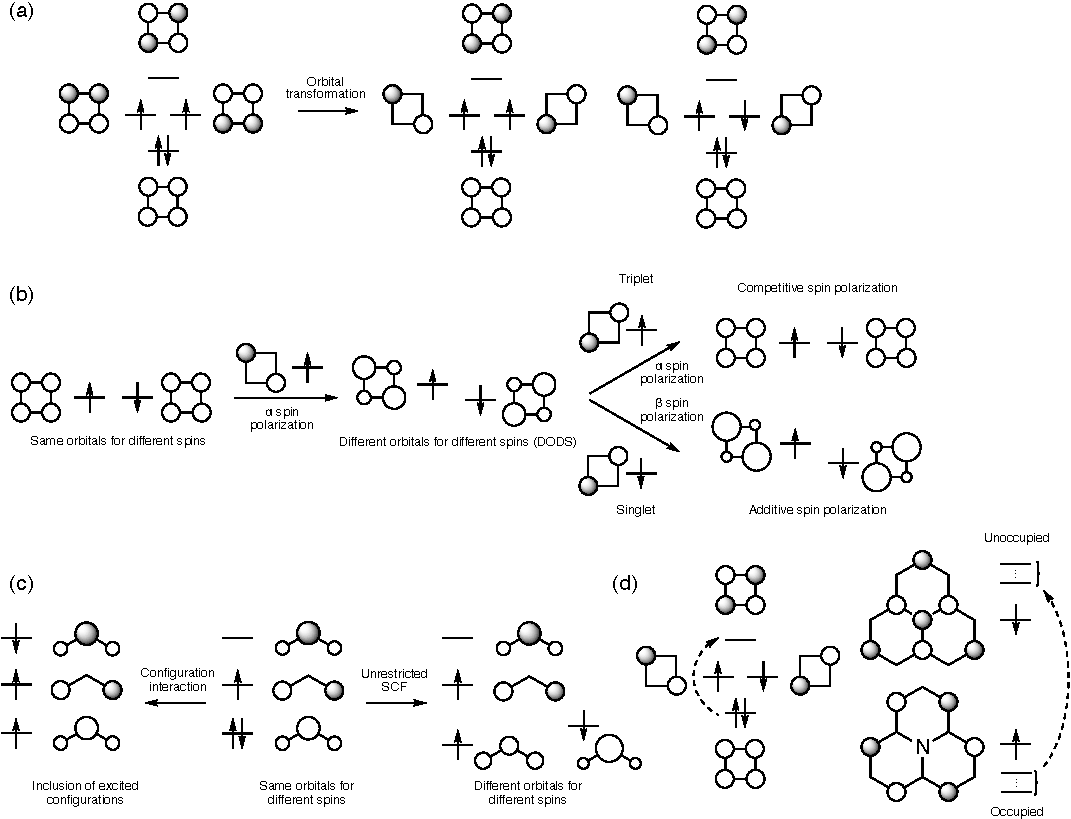
\includegraphics{../data/figures/dynamic_spin_polarization.pdf}

}

\caption{\label{fig-dsp}Dynamic spin polarization stabilizes the
open-shell singlet state over the open-shell triplet. (a) Transformation
of the canonical frontier molecular orbitals creates a set of disjoint
non-bonding molecular orbitals for cyclobutadiene. Singlet and triplet
occupations are shown. (b) Dynamic spin polarization preferentially
stabilizes the singlet state of cyclobutadiene through additive spin
polarization for the singlet and competitive spin polarization for the
triplet. (c) An alternative description of the spin polarization
phenomenon is via configuration interaction and admixture of excited
configurations into the ground state. (d) In the same way as
cyclobutadiene is stabilized by DSP in the singlet ground state,
molecules with inverted singlet-triplet gaps in the excited state are
also stabilized by DSP that can be described by admixture of excited
configurations. For singly excited states, this means addition of doubly
excited states.}

\end{figure}

\[
\DeltaE[DSP]{SCF} =  - \sum_{i}\sum_{k}
    \frac{1}{2} \left( 
    \frac{3 \Integral{-}}{\EState[1]{S} - \EState{S}}
    - \frac{\Integral{-}}{\EState[1]{T} - \EState{T}}
    - \frac{2 \Integral{+}}{\EState[2]{T} - \EState{T}}
    \right)
\]

Here, \(K_x\) and \(K_y\) are exchange operators,
\(E(\phi_{\mathrm{S}})\) and \(E(\phi_{\mathrm{T}})\) are the energies
of the singlet and triplet excited determinants, while
\(E (\phi_{\mathrm{S}}^{1})\), \(E (\phi_{\mathrm{T}}^{1})\) and
\(E(\phi_{\mathrm{T}}^{2})\) are the energies of doubly excited
determinants. They can be written in terms of the correspond orbital
energies, \(\epsilon_i\), provided the same orbitals are used for both
the singlet and triplet
states.\textsuperscript{\protect\hyperlink{ref-benamorSpinPolarizationElectronic2020}{35}}

\[
\DeltaE[DSP]{SCF} =  - \sum_{i}\sum_{k}
    \frac{1}{2} \left( 
    \frac{3 \Integral{-}}{\epsilon_k - \epsilon_i}
    - \frac{\Integral{-}}{\epsilon_k - \epsilon_i}
    - \frac{2 \Integral{+}}{\epsilon_k - \epsilon_i}
    \right)
\]

The simplest approximation for \(\DeltaE{ST}\) taking DSP into account
is then

\[
\DeltaEST[DSP]{SCF} = 2K + \DeltaE[DSP]{SCF}
\]

Alternatively, \(\DeltaE[DSP]{}\) can be calculated with respect to the
CIS
states,\textsuperscript{\protect\hyperlink{ref-head-gordonDoublesCorrectionElectronic1994}{37}}

\[
\begin{split}
\DeltaE[DSP]{CIS} =  - \sum_{i}\sum_{k}
    \frac{1}{2} \left( 
    \frac{3 \Integral{-}}{\epsilon_k + \epsilon_y - \epsilon_y - \epsilon_i - \DeltaE{S,CIS}}
    - \frac{\Integral{-}}{\epsilon_k + \epsilon_y - \epsilon_y - \epsilon_i - \DeltaE{T,CIS}} \right. \\
    \left. - \frac{2 \Integral{+}}{\epsilon_k + \epsilon_y - \epsilon_y - \epsilon_i - \DeltaE{T,CIS}}
    \right)
\end{split}
\]

and added as a correction to the energy gap at the CIS level to yield a
possibly more accurate value

\[
\DeltaEST[DSP]{CIS} = \DeltaEST{CIS} + \DeltaE[DSP]{CIS}
\]

\hypertarget{methods}{%
\section{Methods}\label{methods}}

The PPP method was implemented in the Python package
\textsc{coulson}\textsuperscript{\protect\hyperlink{ref-jornerCoulson}{38}}
which is freely available on GitHub with a permissive MIT license.
Further details on \textsc{coulson} will be reported elsewhere. The PPP
wavefunction was converged with the self-consistent field method using
the naive variational principle. To speed up the calculations, we
derived a spline interpolation of the overlap
integrals,\textsuperscript{\protect\hyperlink{ref-mullikenFormulasNumericalTables1949}{28}}
which will be reported separately. All calculations have been performed
on a MacBook Air laptop computer with an M2 processor. We further
integrated \textsc{coulson} with
\textsc{PySCF}\textsuperscript{\protect\hyperlink{ref-sunRecentDevelopmentsPySCF2020}{39}}
to provide alternative algorithms for the SCF convergence and CIS and
found the results consistent within numerical accuracy. Oscillator
strengths were calculated with the dipole length
approximation.\textsuperscript{\protect\hyperlink{ref-klessingerExcitedStatesPhotochemistry1995}{32},\protect\hyperlink{ref-jorgensenTimedependentHartreeFockCalculations1970}{40},\protect\hyperlink{ref-damourGroundExcitedStateDipole2023}{41}}
Some compounds exhibit negative triplet excitation energies and in some
case even negative singlet excitation energies, which indicates a
restricted-unrestricted instability of the ground state wavefunction. We
have here taken the pragmatic approach to ignore these issues, while we
will highlight below some examples where it occurs and if it has any
effect on the overall results. This approach can be partly justified as
the reference data also does not include any stability analysis. The
results should anyway be indicative of the gap between the lowest
singlet and triplet states with open-shell character, regardless of if
they are lower in energy than the closed-shell singlet.

We used four separate datasets for this study. The first is a set of
azaphenalenes previously studied by some of us, comprising 257
substituted compounds, for which excitation energies were computed with
(2nd-order) algebraic-diagrammatic construction, ADC(2)/{[}Robert: Fill
out{]}, and geometries were optimized with B3LYP/{[}Robert: Fill
out{]}\textsuperscript{\protect\hyperlink{ref-polliceOrganicMoleculesInverted2021}{7}}
The second is a set substituted 138 aza-azulenes with ADC(2)/{[}Robert:
Fill out{]} excitation energies and optimized with the B97-3c composite
method.{[}Robert: Add ref to dataset if it exists.{]} The third is a set
of 16 rationally designed scaffolds, which including substitutions
amounts to 68695 unique compounds, optimized at the B97-3c level and
with excitation energies at the ADC(2)/{[}Robert: Fill out{]}
level.{[}Robert: Add ref to dataset if it exists.{]} The fourth is a set
315 non-alternant hydrocarbons including substitutions, divided into
three subsets of size 76, 187 and 52, optimized at the ωB97X-D/def2-TZVP
level and with excitation energies at the CC2/aug-cc-pVTZ level.

\hypertarget{results-and-discussion}{%
\section{Results and discussion}\label{results-and-discussion}}

\hypertarget{qualitative-understanding-of-the-inverted-gap}{%
\subsection{Qualitative understanding of the inverted
gap}\label{qualitative-understanding-of-the-inverted-gap}}

We first demonstrate that our method is capable of capturing the
inverted \(\DeltaE{ST}\) for some model compounds. As shown by Toyota
and co-workers, pentalene at the ideal \(D_\mathrm{2h}\) geometry has an
inverted gap, while relaxation to the minimum with \(C_\mathrm{2h}\)
symmetry leads to a normal
gap.\textsuperscript{\protect\hyperlink{ref-kosekiViolationHundMultiplicity1985}{5}}
In our calculations, pentalene with equal bond lengths of 1.4 Å displays
a small HOMO-LUMO overlap of 0.24, leading to a small exchange
interaction of only \(2K=\) 2.99 kcal/mol
(Figure~\ref{fig-pentalene-ideal-orbitals}). The dynamic spin
polarization correction \(\DeltaE[DSP]{SCF}\) of -8.96 kcal/mol leads to
a net predicted \(\DeltaEST[DSP]{SCF}\) of -5.97 kcal/mol. Adding
additional correlation with CIS leads to a \(\DeltaEST[DSP]{CIS}\) of
-4.07 kcal/mol. The reference value calculated with ADC(2) is -3.70
kcal/mol. The simple perturbation theory model allows us to gain
additional insight into the contributions to \(\DeltaE[DSP]{SCF}\) as
they correspond to single excitations between doubly occupied orbitals
below the HOMO and unoccupied orbitals above the LUMO
(Figure~\ref{fig-pentalene-ideal-excitations}). Three excitations,
HOMO-3 → LUMO+2, HOMO-2 → LUMO+1 and HOMO-1 → LUMO+3 are identified as
the main contributors to the spin polarization effect, and could
potentially be tuned by substituent effects.

\begin{figure}

{\centering \includegraphics{../results/figures/pentalene_ideal_orbitals.png}

}

\caption{\label{fig-pentalene-ideal-orbitals}Orbitals energies and
frontier orbitals of pentalene at the idealized \(D_\mathrm{2h}\)
geometry and bond lengths of 1.4 Å.}

\end{figure}

\begin{figure}

{\centering \includegraphics{../results/figures/pentalene_ideal_excitations.png}

}

\caption{\label{fig-pentalene-ideal-excitations}Excitations and their
contribution to \(\DeltaE[DSP]{SCF}=\) -8.96 kcal/mol for pentalene at
the \(D_\mathrm{2h}\) geometry and bond lengths of 1.4 Å.}

\end{figure}

Using the relaxed \(C_\mathrm{2h}\) geometry leads to dramatic changes
in the frontier orbitals, with an increased HOMO-LUMO overlap of 0.86
and a sizeable exchange interaction of 15.88 kcal/mol
(Figure~\ref{fig-pentalene-orbitals}). Consequently, the calculated gap
is now normal at \(\DeltaEST[DSP]{SCF}=\) 13.16 kcal/mol, aggravated by
a diminished \(\DeltaE[DSP]{SCF}\) of only -2.72 kcal/mol. A similar
result is obtained with CIS: \(\DeltaEST[DSP]{CIS}=\) 21.08 kcal/mol.
The reference value calculated with ADC(2) is 19.92 kcal/mol. The
excitations contributing to \(\DeltaE[DSP]{SCF}\) at the
\(D_\mathrm{2h}\) geometry have been significantly diminished, only
partially alleviated by the addition of a minor stabilization from
HOMO-2 → LUMO+3 (Figure~\ref{fig-pentalene-excitations}).

\begin{figure}

{\centering \includegraphics{../results/figures/pentalene_orbitals.png}

}

\caption{\label{fig-pentalene-orbitals}Orbitals energies and frontier
orbitals of pentalene at the optimized \(C_\mathrm{2h}\) geometry.}

\end{figure}

\begin{figure}

{\centering \includegraphics{../results/figures/pentalene_excitations.png}

}

\caption{\label{fig-pentalene-excitations}Excitations and their
contribution to \(\DeltaE[DSP]{SCF}=\) -2.72 kcal/mol for pentalene at
the optimized \(C_\mathrm{2h}\) geometry.}

\end{figure}

Azaphenalene is the prototypical molecule that started the renewed
investigations into INVEST molecules, and has been the subject of
numerous studies with high-level quantum chemical methods. Can we
capture the inverted gap, as first measured by Leupin and
Wirz?\textsuperscript{\protect\hyperlink{ref-leupinLowlyingElectronicallyExcited1980}{4}}
The calculations reveal that the HOMO and LUMO are well separated with
spatial overlap of 0.14 and a correspondingly low exchange interaction
of 0.64 kcal/mol (Figure~\ref{fig-azaphenalene-orbitals}). The larger
azaphenalene has 30 excitations that could possibly contribute to the
large \(\DeltaE[DSP]{SCF}\) of -11.34 kcal/mol, but the most import by
far are those from the doubly degenerate HOMO-1 to the doubly degenerate
LUMO+1 (Figure~\ref{fig-azaphenalene-excitations}). In total,
\(\DeltaEST[DSP]{SCF}=\) -10.71 kcal/mol, which is slightly smaller at
the CIS level with \(\DeltaEST[DSP]{CIS}=\) -7.41 kcal/mol.

To conclude this section on the model compounds, our PPP-based protocol
is able to capture the inverted gap, and also provides qualitative
understanding into the physical mechanism of dynamic spin polarization
through identification and visualization of the corresponding
excitations. For these two compounds, the calculated
\(\DeltaEST[DSP]{}\) are more negative at the SCF level compared to CIS.
Compared to ADC(2), it would seem that CIS is preferable, but to
elucidate to which method is better, we now turn to larger datasets.

\begin{figure}

{\centering \includegraphics{../results/figures/azaphenalene_orbitals.png}

}

\caption{\label{fig-azaphenalene-orbitals}Orbitals energies and frontier
orbitals of azaphenalene.}

\end{figure}

\begin{figure}

{\centering \includegraphics{../results/figures/azaphenalene_excitations.png}

}

\caption{\label{fig-azaphenalene-excitations}Excitations and their
contribution to \(\DeltaE[DSP]{SCF}=\) -11.34 kcal/mol for azaphenalene}

\end{figure}

\hypertarget{local-chemical-space-of-azaphenalenes-and-azaazulenes}{%
\subsection{Local chemical space of azaphenalenes and
azaazulenes}\label{local-chemical-space-of-azaphenalenes-and-azaazulenes}}

While our method captures the inverted gap of azaphenalene and
pentalene, it also needs to capture trends with substitution to work
effectively in virtual screening. We therefore calculated 256
substituted azaphenalenes that have previously been studied by some of
us.\textsuperscript{\protect\hyperlink{ref-polliceOrganicMoleculesInverted2021}{7}}
The PPP level S\textsubscript{1} and T\textsubscript{1} excitation
energies are well correlated with those from ADC(2) with \(R^2\) of 0.90
and 0.94, respectively (Figure~\ref{fig-local-azaphenalenes}a,b).
Unfortunately, the oscillator strengths are not as well reproduced with
an \(R^2\) of 0.54, although the Spearman \(\rho\) of 0.82 indicates the
values might be used to rank potential candidates
(Figure~\ref{fig-local-azaphenalenes}c). The problems of obtaining
accurate oscillator strengths at the PPP level of theory are well known
in the literature, and the problem is especially exacerbated with low
oscillator strengths as
here.\textsuperscript{\protect\hyperlink{ref-misurkinElectronicStructureConjugated1974}{42}}.
Crucially, the \(\DeltaE{ST}\) shows good correlations, with \(R^2=\)
0.81 using \(\DeltaEST[DSP]{CIS}\)
(Figure~\ref{fig-local-azaphenalenes}f). This \(R^2\) value is
essentially unchanged from the gap at the CIS level without DSP (0.81,
Figure~\ref{fig-local-azaphenalenes}d) and markedly better than the gap
at the SCF level (0.52, Figure~\ref{fig-local-azaphenalenes}e), showing
the importance of going beyond the SCF level to include at least some
configuration interaction. The results are of similar or better quality
achieved by Pernal and co-workers for different set of azaphenalenes
using SCF + DSP with orbitals from
DFT.\textsuperscript{\protect\hyperlink{ref-drwalRoleSpinPolarization2023}{36}}
To further analyze the results in terms of a binary classification into
normal/inverted, we calculated the true positives (TP), true negatives
(TN), false positives (FP) and false negatives (FN), as well as a range
of common classification scores (Table~\ref{tbl-local-azaphenalenes}).
The most important metrics for virtual screening are, in our opinion,
the recall and the specificity. The recall measures the fraction of
inverted molecules that the protocol captures, and is 0.58 at the SCF
level and 0.56 at the CIS level. The specificity measures the fraction
of non-inverted molecules that the protocol identifies, and is 0.94 at
the SCF level and 0.97 at the CIS level. This metrics mean that we are
able to capture a large proportion of the molecules with inverted gaps,
while filtering out most non-inverted molecules. The results for these
azaphenalenes clearly indicate that the PPP protocol could be used to
prescreen candidates of this compound class for \(\DeltaE{ST}\), while
further pruning with another method is likely needed for the oscillator
strengths.

\begin{figure}

{\centering \includegraphics{../results/figures/local_azaphenalenes.pdf}

}

\caption{\label{fig-local-azaphenalenes}Excitation properties for
azaphenalenes \emph{vs.} the reference level. (a) Singlet excitation
energies. (b) Triplet excitation energies. (c) Oscillator strengths. (d)
Singlet-triplet energy gaps with CIS. (e) Singlet-triplet energy gaps
with SCF + DSP. (f) Singlet-triplet energy gaps with CIS + DSP.}

\end{figure}

\hypertarget{tbl-local-azaphenalenes}{}
\begin{longtable}[]{@{}
  >{\raggedright\arraybackslash}p{(\columnwidth - 22\tabcolsep) * \real{0.0490}}
  >{\raggedleft\arraybackslash}p{(\columnwidth - 22\tabcolsep) * \real{0.0882}}
  >{\raggedleft\arraybackslash}p{(\columnwidth - 22\tabcolsep) * \real{0.0980}}
  >{\raggedleft\arraybackslash}p{(\columnwidth - 22\tabcolsep) * \real{0.0588}}
  >{\raggedleft\arraybackslash}p{(\columnwidth - 22\tabcolsep) * \real{0.1078}}
  >{\raggedleft\arraybackslash}p{(\columnwidth - 22\tabcolsep) * \real{0.1176}}
  >{\raggedleft\arraybackslash}p{(\columnwidth - 22\tabcolsep) * \real{0.0980}}
  >{\raggedleft\arraybackslash}p{(\columnwidth - 22\tabcolsep) * \real{0.1471}}
  >{\raggedleft\arraybackslash}p{(\columnwidth - 22\tabcolsep) * \real{0.0588}}
  >{\raggedleft\arraybackslash}p{(\columnwidth - 22\tabcolsep) * \real{0.0588}}
  >{\raggedleft\arraybackslash}p{(\columnwidth - 22\tabcolsep) * \real{0.0588}}
  >{\raggedleft\arraybackslash}p{(\columnwidth - 22\tabcolsep) * \real{0.0588}}@{}}
\caption{\label{tbl-local-azaphenalenes}Metrics for
azaphenalenes.}\tabularnewline
\toprule()
\begin{minipage}[b]{\linewidth}\raggedright
\end{minipage} & \begin{minipage}[b]{\linewidth}\raggedleft
\(R^2\)
\end{minipage} & \begin{minipage}[b]{\linewidth}\raggedleft
\(\rho\)
\end{minipage} & \begin{minipage}[b]{\linewidth}\raggedleft
F1
\end{minipage} & \begin{minipage}[b]{\linewidth}\raggedleft
ROC-AUC
\end{minipage} & \begin{minipage}[b]{\linewidth}\raggedleft
Accuracy
\end{minipage} & \begin{minipage}[b]{\linewidth}\raggedleft
Recall
\end{minipage} & \begin{minipage}[b]{\linewidth}\raggedleft
Specificity
\end{minipage} & \begin{minipage}[b]{\linewidth}\raggedleft
TP
\end{minipage} & \begin{minipage}[b]{\linewidth}\raggedleft
TN
\end{minipage} & \begin{minipage}[b]{\linewidth}\raggedleft
FP
\end{minipage} & \begin{minipage}[b]{\linewidth}\raggedleft
FN
\end{minipage} \\
\midrule()
\endfirsthead
\toprule()
\begin{minipage}[b]{\linewidth}\raggedright
\end{minipage} & \begin{minipage}[b]{\linewidth}\raggedleft
\(R^2\)
\end{minipage} & \begin{minipage}[b]{\linewidth}\raggedleft
\(\rho\)
\end{minipage} & \begin{minipage}[b]{\linewidth}\raggedleft
F1
\end{minipage} & \begin{minipage}[b]{\linewidth}\raggedleft
ROC-AUC
\end{minipage} & \begin{minipage}[b]{\linewidth}\raggedleft
Accuracy
\end{minipage} & \begin{minipage}[b]{\linewidth}\raggedleft
Recall
\end{minipage} & \begin{minipage}[b]{\linewidth}\raggedleft
Specificity
\end{minipage} & \begin{minipage}[b]{\linewidth}\raggedleft
TP
\end{minipage} & \begin{minipage}[b]{\linewidth}\raggedleft
TN
\end{minipage} & \begin{minipage}[b]{\linewidth}\raggedleft
FP
\end{minipage} & \begin{minipage}[b]{\linewidth}\raggedleft
FN
\end{minipage} \\
\midrule()
\endhead
SCF & 0.52 & 0.72 & 0.73 & 0.76 & 0.62 & 0.58 & 0.94 & 128 & 32 & 2 &
94 \\
CIS & 0.81 & 0.83 & 0.72 & 0.77 & 0.62 & 0.56 & 0.97 & 125 & 33 & 1 &
97 \\
\bottomrule()
\end{longtable}

While we see success for the azaphenalenes, the situation for the
azulenes is unfortunately worse. The PPP level S\textsubscript{1} and
T\textsubscript{1} excitation energies are only moderately correlated
with those from ADC(2) with \(R^2\) of 0.44 and 0.47, respectively
(Figure~\ref{fig-local-azulenes}a,b). For the oscillator strengths, the
situation is rather catastrophic with \(R^2\) of 0.00 implying no
correlation whatsoever (Figure~\ref{fig-local-azulenes}c). The situation
for the \(\DeltaE{ST}\) also worse than for the azaphenalenes, with
\(R^2=\) 0.46 with CIS + DSP, a marked improvement on 0.18 with SCF +
DSP (Figure~\ref{fig-local-azulenes}e,f). Unfortunately, the negative
gaps are not recovered, leading to recalls of 0.00 as none of five
inverted molecules could be identified (Table~\ref{tbl-local-azulenes}).
It could be speculated that the worse performance for the azulenes comes
from the fact that they are non-alternants, for which the approximations
are expected to be less applicable. Considering the contrasting
performance for the azaphenalenes and azulenes, it seems clear that the
PPP screening protocol will inevitably miss some hits belonging to
particular compound classes. To investigate the global performance of
the model we turned to a more diverse set with 16 different compound
classes.

\begin{figure}

{\centering \includegraphics{../results/figures/local_azulenes.pdf}

}

\caption{\label{fig-local-azulenes}Excitation properties for azaazulenes
\emph{vs.} the reference level. (a) Singlet excitation energies. (b)
Triplet excitation energies. (c) Oscillator strengths. (d)
Singlet-triplet energy gaps with CIS. (e) Singlet-triplet energy gaps
with SCF + DSP. (f) Singlet-triplet energy gaps with CIS + DSP.}

\end{figure}

\hypertarget{tbl-local-azulenes}{}
\begin{longtable}[]{@{}
  >{\raggedright\arraybackslash}p{(\columnwidth - 22\tabcolsep) * \real{0.0490}}
  >{\raggedleft\arraybackslash}p{(\columnwidth - 22\tabcolsep) * \real{0.0882}}
  >{\raggedleft\arraybackslash}p{(\columnwidth - 22\tabcolsep) * \real{0.0980}}
  >{\raggedleft\arraybackslash}p{(\columnwidth - 22\tabcolsep) * \real{0.0588}}
  >{\raggedleft\arraybackslash}p{(\columnwidth - 22\tabcolsep) * \real{0.1078}}
  >{\raggedleft\arraybackslash}p{(\columnwidth - 22\tabcolsep) * \real{0.1176}}
  >{\raggedleft\arraybackslash}p{(\columnwidth - 22\tabcolsep) * \real{0.0980}}
  >{\raggedleft\arraybackslash}p{(\columnwidth - 22\tabcolsep) * \real{0.1471}}
  >{\raggedleft\arraybackslash}p{(\columnwidth - 22\tabcolsep) * \real{0.0588}}
  >{\raggedleft\arraybackslash}p{(\columnwidth - 22\tabcolsep) * \real{0.0588}}
  >{\raggedleft\arraybackslash}p{(\columnwidth - 22\tabcolsep) * \real{0.0588}}
  >{\raggedleft\arraybackslash}p{(\columnwidth - 22\tabcolsep) * \real{0.0588}}@{}}
\caption{\label{tbl-local-azulenes}Metrics for
azaazulenes.}\tabularnewline
\toprule()
\begin{minipage}[b]{\linewidth}\raggedright
\end{minipage} & \begin{minipage}[b]{\linewidth}\raggedleft
\(R^2\)
\end{minipage} & \begin{minipage}[b]{\linewidth}\raggedleft
\(\rho\)
\end{minipage} & \begin{minipage}[b]{\linewidth}\raggedleft
F1
\end{minipage} & \begin{minipage}[b]{\linewidth}\raggedleft
ROC-AUC
\end{minipage} & \begin{minipage}[b]{\linewidth}\raggedleft
Accuracy
\end{minipage} & \begin{minipage}[b]{\linewidth}\raggedleft
Recall
\end{minipage} & \begin{minipage}[b]{\linewidth}\raggedleft
Specificity
\end{minipage} & \begin{minipage}[b]{\linewidth}\raggedleft
TP
\end{minipage} & \begin{minipage}[b]{\linewidth}\raggedleft
TN
\end{minipage} & \begin{minipage}[b]{\linewidth}\raggedleft
FP
\end{minipage} & \begin{minipage}[b]{\linewidth}\raggedleft
FN
\end{minipage} \\
\midrule()
\endfirsthead
\toprule()
\begin{minipage}[b]{\linewidth}\raggedright
\end{minipage} & \begin{minipage}[b]{\linewidth}\raggedleft
\(R^2\)
\end{minipage} & \begin{minipage}[b]{\linewidth}\raggedleft
\(\rho\)
\end{minipage} & \begin{minipage}[b]{\linewidth}\raggedleft
F1
\end{minipage} & \begin{minipage}[b]{\linewidth}\raggedleft
ROC-AUC
\end{minipage} & \begin{minipage}[b]{\linewidth}\raggedleft
Accuracy
\end{minipage} & \begin{minipage}[b]{\linewidth}\raggedleft
Recall
\end{minipage} & \begin{minipage}[b]{\linewidth}\raggedleft
Specificity
\end{minipage} & \begin{minipage}[b]{\linewidth}\raggedleft
TP
\end{minipage} & \begin{minipage}[b]{\linewidth}\raggedleft
TN
\end{minipage} & \begin{minipage}[b]{\linewidth}\raggedleft
FP
\end{minipage} & \begin{minipage}[b]{\linewidth}\raggedleft
FN
\end{minipage} \\
\midrule()
\endhead
SCF & 0.18 & 0.41 & nan & 0.50 & 0.96 & 0.00 & 1.00 & 0 & 133 & 0 & 5 \\
CIS & 0.46 & 0.65 & nan & 0.50 & 0.96 & 0.00 & 1.00 & 0 & 133 & 0 & 5 \\
\bottomrule()
\end{longtable}

\hypertarget{screening-widely}{%
\subsection{Screening widely}\label{screening-widely}}

Here we used a dataset previously generated by some of us using rational
design rules, comprising 16 different molecular scaffolds, the details
of which will be presented elsewhere. Out of 68695 compounds, only 5
failed, which corresponds to a success rate of 99.99. The total runtime
using four cores on the M2 processor was 12.61 CPU hours. The
S\textsubscript{1} and T\textsubscript{1} excitation energies are fairly
reproduced with (Figure~\ref{fig-global-all}a,b) \(R^2\) of 0.66 and
0.70 vs ADC(2), respectively. As seen in
Figure~\ref{fig-global-all-gaps}a, the \(\DeltaE{ST}\) at the SCF + DSP
level shows a moderate \(R^2\) of 0.46, which increases significantly to
0.71 at the CIS + DSP level (Figure~\ref{fig-global-all-gaps}b).
However, due to a systematic overestimation of \(\DeltaE{ST}\), the F1
score is still low at 0.27 and a poor recall of 0.16
(Table~\ref{tbl-global-all}). We therefore added a linear correction
\(\DeltaEST[DSP]{CIS,LC}=\) 0.53 \(\times\DeltaEST[DSP]{CIS}\) -0.15,
which increases the F1 score to 0.55 and the recall to 0.51
(Figure~\ref{fig-global-all-gaps}c). The specificity simultaneously
decreases from 0.99 to 0.96, but overall the linear correction would be
preferable for virtual screening where there is a stronger focus on
finding rare hits. Applying the linear correction to the azaphenalenes
(Figure~\ref{fig-local-corr}a) and (Figure~\ref{fig-local-corr}b) leads
to an improvement in the recall of the former from 0.56 to 0.94 while
still none of the inverted azulenes are recovered. The oscillator
strengths are unfortunately poorly correlated for the rational design
set, with \(R^2=\) 0.21, although the Spearman rank correlation is more
encouraging at 0.58 (Figure~\ref{fig-global-all}c). Taken together, the
results reinforce the conclusions from the case study of the
azaphenalenes, that the PPP protocol is suitable for screening
\(\DeltaE{ST}\) while it struggles for oscillator strengths.

A more detailed breakdown of the correlations into the different
scaffolds shows that the highest \(R^2\) of 0.82 is obtained for
dicyclopenta{[}a,e{]}cyclooctene, while the lowest is obtained for
bowtiene with 0.07. For recall, the corresponding range is 0.92 for
zurlene to 0.01 for phenazulene. The wide range in \(R^2\) and recall
further reinforces that the method struggles with some particular
compounds classes despite its favorable global performance. Despite
these problems, the method is able to capture inverted molecules in 15
out of the 15 scaffolds where they occur. Even for the azulenes included
in this screening set at least some candidates are found, in contrast to
the findings above for the azaazulenes. The per-scaffold oscillator
strengths are arguably sufficiently good to allow for local screening in
some cases (Figure~\ref{fig-global-scaffolds-oscillator}). The
per-scaffold S\textsubscript{1} and T\textsubscript{1} excitation
energies can be found in (Figure~\ref{fig-global-scaffolds-singlet}) and
(Figure~\ref{fig-global-scaffolds-triplet}), respectively. Notable
failures are for cyclobuta-1,3-diene with \(R^2\) of 0.29 and 0.27,
respectively, and phenazulene and dicyclopenta{[}a,c{]}cyclooctene,
where some negative T\textsubscript{1} excitation energies indicate
restricted-unrestricted instabilities.

\begin{figure}

{\centering \includegraphics{../results/figures/global_all_gaps.pdf}

}

\caption{\label{fig-global-all-gaps}Singlet-triplet energy gaps for
rationally design set \emph{vs.} reference level for (a) SCF + DSP, (b)
CIS + DSP and (c) CIS + DSP and linear correction.}

\end{figure}

\hypertarget{tbl-global-all}{}
\begin{longtable}[]{@{}
  >{\raggedright\arraybackslash}p{(\columnwidth - 22\tabcolsep) * \real{0.1404}}
  >{\raggedleft\arraybackslash}p{(\columnwidth - 22\tabcolsep) * \real{0.0789}}
  >{\raggedleft\arraybackslash}p{(\columnwidth - 22\tabcolsep) * \real{0.0877}}
  >{\raggedleft\arraybackslash}p{(\columnwidth - 22\tabcolsep) * \real{0.0526}}
  >{\raggedleft\arraybackslash}p{(\columnwidth - 22\tabcolsep) * \real{0.0965}}
  >{\raggedleft\arraybackslash}p{(\columnwidth - 22\tabcolsep) * \real{0.1053}}
  >{\raggedleft\arraybackslash}p{(\columnwidth - 22\tabcolsep) * \real{0.0877}}
  >{\raggedleft\arraybackslash}p{(\columnwidth - 22\tabcolsep) * \real{0.1316}}
  >{\raggedleft\arraybackslash}p{(\columnwidth - 22\tabcolsep) * \real{0.0526}}
  >{\raggedleft\arraybackslash}p{(\columnwidth - 22\tabcolsep) * \real{0.0614}}
  >{\raggedleft\arraybackslash}p{(\columnwidth - 22\tabcolsep) * \real{0.0526}}
  >{\raggedleft\arraybackslash}p{(\columnwidth - 22\tabcolsep) * \real{0.0526}}@{}}
\caption{\label{tbl-global-all}Metrics for rationally designed
set.}\tabularnewline
\toprule()
\begin{minipage}[b]{\linewidth}\raggedright
\end{minipage} & \begin{minipage}[b]{\linewidth}\raggedleft
\(R^2\)
\end{minipage} & \begin{minipage}[b]{\linewidth}\raggedleft
\(\rho\)
\end{minipage} & \begin{minipage}[b]{\linewidth}\raggedleft
F1
\end{minipage} & \begin{minipage}[b]{\linewidth}\raggedleft
ROC-AUC
\end{minipage} & \begin{minipage}[b]{\linewidth}\raggedleft
Accuracy
\end{minipage} & \begin{minipage}[b]{\linewidth}\raggedleft
Recall
\end{minipage} & \begin{minipage}[b]{\linewidth}\raggedleft
Specificity
\end{minipage} & \begin{minipage}[b]{\linewidth}\raggedleft
TP
\end{minipage} & \begin{minipage}[b]{\linewidth}\raggedleft
TN
\end{minipage} & \begin{minipage}[b]{\linewidth}\raggedleft
FP
\end{minipage} & \begin{minipage}[b]{\linewidth}\raggedleft
FN
\end{minipage} \\
\midrule()
\endfirsthead
\toprule()
\begin{minipage}[b]{\linewidth}\raggedright
\end{minipage} & \begin{minipage}[b]{\linewidth}\raggedleft
\(R^2\)
\end{minipage} & \begin{minipage}[b]{\linewidth}\raggedleft
\(\rho\)
\end{minipage} & \begin{minipage}[b]{\linewidth}\raggedleft
F1
\end{minipage} & \begin{minipage}[b]{\linewidth}\raggedleft
ROC-AUC
\end{minipage} & \begin{minipage}[b]{\linewidth}\raggedleft
Accuracy
\end{minipage} & \begin{minipage}[b]{\linewidth}\raggedleft
Recall
\end{minipage} & \begin{minipage}[b]{\linewidth}\raggedleft
Specificity
\end{minipage} & \begin{minipage}[b]{\linewidth}\raggedleft
TP
\end{minipage} & \begin{minipage}[b]{\linewidth}\raggedleft
TN
\end{minipage} & \begin{minipage}[b]{\linewidth}\raggedleft
FP
\end{minipage} & \begin{minipage}[b]{\linewidth}\raggedleft
FN
\end{minipage} \\
\midrule()
\endhead
SCF + DSP & 0.46 & 0.60 & 0.40 & 0.63 & 0.91 & 0.27 & 0.99 & 2073 &
60490 & 561 & 5566 \\
CIS + DSP & 0.71 & 0.85 & 0.27 & 0.58 & 0.90 & 0.16 & 0.99 & 1227 &
60736 & 315 & 6412 \\
CIS + DSP + LC & 0.71 & 0.85 & 0.55 & 0.73 & 0.91 & 0.51 & 0.96 & 3867 &
58592 & 2459 & 3772 \\
\bottomrule()
\end{longtable}

\hypertarget{external-validation}{%
\subsection{External validation}\label{external-validation}}

To further test the validity of the method, we calculated a series of
compounds recently published by Garner \emph{et.
al}.\textsuperscript{\protect\hyperlink{ref-garnerDoublebondDelocalizationNonalternant2023}{11}}
The dataset comes in three parts: (1) non-alternants, (2) non-alternants
with constrained high-symmetry geometries (we here follow the original
terminology and call these ``avoided symmetry'') and (3) substituted
non-alternants (here called ``substituted''). Out of the substituted
compounds, four could not be calculated as they contain four-coordinate
P atoms for which our PPP model lacks parameters. We here opted to use
the CC2/aug-cc-pVDZ data from the original paper as reference as it is
the highest level which has the most complete coverage of the dataset.

Our computed \(\DeltaE{ST}\) with the linearly corrected CIS + DSP show
fair correlations with the CC2 values, with \(R^2\)s of 0.68, 0.69 and
0.56, respectively (Figure~\ref{fig-garner-gaps}). Gratifyingly, the
recalls are 0.50, 0.80 and 0.74, respectively, showing that we can
recover a large part of the inverted molecules found with the much more
expensive CC2 method (Table~\ref{tbl-garner-gaps}). Although some of the
compounds are also present in the rationally designed set that we used
for the linear correction above, we believe that they are not
sufficiently many to compromise the use of the Garner data as external
validation (Figure~\ref{fig-garner-gaps}). We also indicate in the plots
which compounds show instabilities (Figure~\ref{fig-garner-gaps}). There
seems to be no clear deterioration in the performance, although also the
reference data might exhibit instabilities as there is no mention of any
stability analysis in the original
manuscript.\textsuperscript{\protect\hyperlink{ref-garnerDoublebondDelocalizationNonalternant2023}{11}}

In summary, the external validation shows that the PPP method can
recover inverted molecules at a fraction of the cost of more expensive
methods such as CC2.

\begin{figure}

{\centering \includegraphics{../results/figures/garner_gaps.pdf}

}

\caption{\label{fig-garner-gaps}Singlet-triplet energy gaps for CIS +
DSP and linear correction \emph{vs.} reference level for the subsets of
(a) non-alternants (b) non-alternants constrained to higher symmetry and
(c) substituted non-alternants. Compounds contained in the rationally
designed sets are marked with dashed circles and those with negative
triplet excitation energies are marked with a semi-transparent red
circle.}

\end{figure}

\hypertarget{tbl-garner-gaps}{}
\begin{longtable}[]{@{}
  >{\raggedright\arraybackslash}p{(\columnwidth - 22\tabcolsep) * \real{0.1565}}
  >{\raggedleft\arraybackslash}p{(\columnwidth - 22\tabcolsep) * \real{0.0783}}
  >{\raggedleft\arraybackslash}p{(\columnwidth - 22\tabcolsep) * \real{0.0870}}
  >{\raggedleft\arraybackslash}p{(\columnwidth - 22\tabcolsep) * \real{0.0522}}
  >{\raggedleft\arraybackslash}p{(\columnwidth - 22\tabcolsep) * \real{0.0957}}
  >{\raggedleft\arraybackslash}p{(\columnwidth - 22\tabcolsep) * \real{0.1043}}
  >{\raggedleft\arraybackslash}p{(\columnwidth - 22\tabcolsep) * \real{0.0870}}
  >{\raggedleft\arraybackslash}p{(\columnwidth - 22\tabcolsep) * \real{0.1304}}
  >{\raggedleft\arraybackslash}p{(\columnwidth - 22\tabcolsep) * \real{0.0522}}
  >{\raggedleft\arraybackslash}p{(\columnwidth - 22\tabcolsep) * \real{0.0522}}
  >{\raggedleft\arraybackslash}p{(\columnwidth - 22\tabcolsep) * \real{0.0522}}
  >{\raggedleft\arraybackslash}p{(\columnwidth - 22\tabcolsep) * \real{0.0522}}@{}}
\caption{\label{tbl-garner-gaps}Metrics for the dataset from Garner
\emph{et al.}}\tabularnewline
\toprule()
\begin{minipage}[b]{\linewidth}\raggedright
\end{minipage} & \begin{minipage}[b]{\linewidth}\raggedleft
\(R^2\)
\end{minipage} & \begin{minipage}[b]{\linewidth}\raggedleft
\(\rho\)
\end{minipage} & \begin{minipage}[b]{\linewidth}\raggedleft
F1
\end{minipage} & \begin{minipage}[b]{\linewidth}\raggedleft
ROC-AUC
\end{minipage} & \begin{minipage}[b]{\linewidth}\raggedleft
Accuracy
\end{minipage} & \begin{minipage}[b]{\linewidth}\raggedleft
Recall
\end{minipage} & \begin{minipage}[b]{\linewidth}\raggedleft
Specificity
\end{minipage} & \begin{minipage}[b]{\linewidth}\raggedleft
TP
\end{minipage} & \begin{minipage}[b]{\linewidth}\raggedleft
TN
\end{minipage} & \begin{minipage}[b]{\linewidth}\raggedleft
FP
\end{minipage} & \begin{minipage}[b]{\linewidth}\raggedleft
FN
\end{minipage} \\
\midrule()
\endfirsthead
\toprule()
\begin{minipage}[b]{\linewidth}\raggedright
\end{minipage} & \begin{minipage}[b]{\linewidth}\raggedleft
\(R^2\)
\end{minipage} & \begin{minipage}[b]{\linewidth}\raggedleft
\(\rho\)
\end{minipage} & \begin{minipage}[b]{\linewidth}\raggedleft
F1
\end{minipage} & \begin{minipage}[b]{\linewidth}\raggedleft
ROC-AUC
\end{minipage} & \begin{minipage}[b]{\linewidth}\raggedleft
Accuracy
\end{minipage} & \begin{minipage}[b]{\linewidth}\raggedleft
Recall
\end{minipage} & \begin{minipage}[b]{\linewidth}\raggedleft
Specificity
\end{minipage} & \begin{minipage}[b]{\linewidth}\raggedleft
TP
\end{minipage} & \begin{minipage}[b]{\linewidth}\raggedleft
TN
\end{minipage} & \begin{minipage}[b]{\linewidth}\raggedleft
FP
\end{minipage} & \begin{minipage}[b]{\linewidth}\raggedleft
FN
\end{minipage} \\
\midrule()
\endhead
Non-alternants & 0.68 & 0.78 & 0.67 & 0.75 & 0.97 & 0.50 & 1.00 & 2 & 75
& 0 & 2 \\
Avoided symmetry & 0.69 & 0.84 & 0.83 & 0.87 & 0.89 & 0.80 & 0.94 & 12 &
30 & 2 & 3 \\
Substituted & 0.56 & 0.78 & 0.80 & 0.85 & 0.90 & 0.74 & 0.96 & 14 & 50 &
2 & 5 \\
\bottomrule()
\end{longtable}

\hypertarget{conclusions-and-outlook}{%
\section{Conclusions and outlook}\label{conclusions-and-outlook}}

To conclude, we have shown that the Pariser-Parr-Pople theory, a simple
semi-empirical \(\pi\)-electron theory with a minimal basis, can be used
to screen for molecules with inverted singlet-triplets energy gaps, both
locally and globally. Unfortunately, the method does not seem capable of
screening for oscillator strengths with the same accuracy, with
exceptions for some scaffolds. The chief limitation of the method is
that it only includes the \(\pi\)-electron system and therefore
struggles with: (1) functional groups without a clear
\(\sigma\)--\(\pi\) separation (found in common functional groups such
as sulfonyls) (2) inductive effects and (3) neglect of
\(n \rightarrow \pi^*\) transitions. Further limitations include (4)
lack of solvation model and need for (5) already optimized geometries.
We believe that at at least some of these limitations could be mitigated
by a reparametrization specifically targeting inverted gaps, while
geometries from the fast GFN-xTB method would be suitable.

Taken together, we foresee that the presented methodology can be used
for ultrahigh-throughput virtual screening campaigns and in inverse
design algorithms, followed by curation of hits using more accurate
quantum-chemical methods. Active learning schemes could also be used
with machine learning corrections to the PPP singlet-triplet gaps. The
method has great potential to accelerate the discovery of the next
generation of OLED materials based on INVEST.

\hypertarget{acknowledgements}{%
\section{Acknowledgements}\label{acknowledgements}}

K.J. acknowledges funding through an International Postdoc grant from
the Swedish Research Council (No.~2020-00314). A. A.-G. acknowledges
support of Natural Resources Canada and the Canada 150 Research Chairs
program and CIFAR, as well as the generous support of Anders G. Frøseth.

\hypertarget{references}{%
\section{References}\label{references}}

\hypertarget{refs}{}
\begin{CSLReferences}{0}{0}
\leavevmode\vadjust pre{\hypertarget{ref-yangRecentAdvancesOrganic2017}{}}%
\CSLLeftMargin{(1) }%
\CSLRightInline{Yang, Z.; Mao, Z.; Xie, Z.; Zhang, Y.; Liu, S.; Zhao,
J.; Xu, J.; Chi, Z.; Aldred, M. P. Recent Advances in Organic Thermally
Activated Delayed Fluorescence Materials. \emph{Chem. Soc. Rev.}
\textbf{2017}, \emph{46} (3), 915--1016.
\url{https://doi.org/10.1039/C6CS00368K}.}

\leavevmode\vadjust pre{\hypertarget{ref-liOrganicMoleculesInverted2022}{}}%
\CSLLeftMargin{(2) }%
\CSLRightInline{Li, J.; Li, Z.; Liu, H.; Gong, H.; Zhang, J.; Yao, Y.;
Guo, Q. Organic Molecules with Inverted Singlet-Triplet Gaps.
\emph{Front. Chem.} \textbf{2022}, \emph{10}, 999856.
\url{https://doi.org/10.3389/fchem.2022.999856}.}

\leavevmode\vadjust pre{\hypertarget{ref-kollmarViolationHundRule1978}{}}%
\CSLLeftMargin{(3) }%
\CSLRightInline{Kollmar, H.; Staemmler, V. Violation of {Hund}'s Rule by
Spin Polarization in Molecules. \emph{Theoret. Chim. Acta}
\textbf{1978}, \emph{48} (3), 223--239.
\url{https://doi.org/10.1007/BF00549021}.}

\leavevmode\vadjust pre{\hypertarget{ref-leupinLowlyingElectronicallyExcited1980}{}}%
\CSLLeftMargin{(4) }%
\CSLRightInline{Leupin, W.; Wirz, J. Low-Lying Electronically Excited
States of Cycl{[}3.3.3{]}azine, a Bridged 12π-Perimeter. \emph{J. Am.
Chem. Soc.} \textbf{1980}, \emph{102} (19), 6068--6075.
\url{https://doi.org/10.1021/ja00539a016}.}

\leavevmode\vadjust pre{\hypertarget{ref-kosekiViolationHundMultiplicity1985}{}}%
\CSLLeftMargin{(5) }%
\CSLRightInline{Koseki, S.; Nakajima, T.; Toyota, A. Violation of
{Hund}'s Multiplicity Rule in the Electronically Excited States of
Conjugated Hydrocarbons. \emph{Can. J. Chem.} \textbf{1985}, \emph{63}
(7), 1572--1579. \url{https://doi.org/10.1139/v85-267}.}

\leavevmode\vadjust pre{\hypertarget{ref-desilvaInvertedSingletTriplet2019}{}}%
\CSLLeftMargin{(6) }%
\CSLRightInline{de Silva, P. Inverted {Singlet}--{Triplet Gaps} and
{Their Relevance} to {Thermally Activated Delayed Fluorescence}.
\emph{J. Phys. Chem. Lett.} \textbf{2019}, \emph{10} (18), 5674--5679.
\url{https://doi.org/10.1021/acs.jpclett.9b02333}.}

\leavevmode\vadjust pre{\hypertarget{ref-polliceOrganicMoleculesInverted2021}{}}%
\CSLLeftMargin{(7) }%
\CSLRightInline{Pollice, R.; Friederich, P.; Lavigne, C.; Gomes, G. dos
P.; Aspuru-Guzik, A. Organic Molecules with Inverted Gaps Between First
Excited Singlet and Triplet States and Appreciable Fluorescence Rates.
\emph{Matter} \textbf{2021}, \emph{4} (5), 1654--1682.
\url{https://doi.org/10.1016/j.matt.2021.02.017}.}

\leavevmode\vadjust pre{\hypertarget{ref-aizawaDelayedFluorescenceInverted2022}{}}%
\CSLLeftMargin{(8) }%
\CSLRightInline{Aizawa, N.; Pu, Y.-J.; Harabuchi, Y.; Nihonyanagi, A.;
Ibuka, R.; Inuzuka, H.; Dhara, B.; Koyama, Y.; Nakayama, K.; Maeda, S.;
Araoka, F.; Miyajima, D. Delayed Fluorescence from Inverted Singlet and
Triplet Excited States. \emph{Nature} \textbf{2022}, \emph{609} (7927),
502--506. \url{https://doi.org/10.1038/s41586-022-05132-y}.}

\leavevmode\vadjust pre{\hypertarget{ref-terenceblaskovitsSymmetryInducedSinglet2023}{}}%
\CSLLeftMargin{(9) }%
\CSLRightInline{Terence Blaskovits, J.; Garner, M. H.; Corminboeuf, C.
Symmetry‐{Induced Singlet}‐{Triplet Inversions} in {Non}‐{Alternant
Hydrocarbons}**. \emph{Angew. Chem. Int. Ed.} \textbf{2023}, \emph{62}
(15), e202218156. \url{https://doi.org/10.1002/anie.202218156}.}

\leavevmode\vadjust pre{\hypertarget{ref-omarIdentificationUnknownInverted2023}{}}%
\CSLLeftMargin{(10) }%
\CSLRightInline{Omar, O.; Xie, X.; Troisi, A.; Padula, D.
\emph{Identification of {Unknown Inverted Singlet-Triplet Cores} by
{High--Throughput Virtual Screening}}.
\url{https://doi.org/10.26434/chemrxiv-2023-h7tsp-v3}.}

\leavevmode\vadjust pre{\hypertarget{ref-garnerDoublebondDelocalizationNonalternant2023}{}}%
\CSLLeftMargin{(11) }%
\CSLRightInline{Garner, M. H.; Blaskovits, J. T.; Corminboeuf, C.
\emph{Double-bond delocalization in non-alternant hydrocarbons induces
inverted singlet-triplet gaps}.
\url{https://doi.org/10.26434/chemrxiv-2023-568ks}.}

\leavevmode\vadjust pre{\hypertarget{ref-casidaProgressTimeDependentDensityFunctional2012}{}}%
\CSLLeftMargin{(12) }%
\CSLRightInline{Casida, M. E.; Huix-Rotllant, M.
\href{http://www.annualreviews.org/doi/full/10.1146/annurev-physchem-032511-143803}{Progress
in {Time-Dependent Density-Functional Theory}}. \emph{Annu. Rev. Phys.
Chem.} \textbf{2012}, \emph{63}, 287--323.}

\leavevmode\vadjust pre{\hypertarget{ref-ricciSingletTripletExcited2021}{}}%
\CSLLeftMargin{(13) }%
\CSLRightInline{Ricci, G.; San‐Fabián, E.; Olivier, Y.; Sancho‐García,
J. C. Singlet‐{Triplet Excited}‐{State Inversion} in {Heptazine} and
{Related Molecules}: {Assessment} of {TD}‐{DFT} and {\emph{Ab Initio}}
{Methods}. \emph{ChemPhysChem} \textbf{2021}, cphc.202000926.
\url{https://doi.org/10.1002/cphc.202000926}.}

\leavevmode\vadjust pre{\hypertarget{ref-sancho-garciaViolationHundRule2022}{}}%
\CSLLeftMargin{(14) }%
\CSLRightInline{Sancho-García, J. C.; Brémond, E.; Ricci, G.;
Pérez-Jiménez, A. J.; Olivier, Y.; Adamo, C. Violation of {Hund}'s Rule
in Molecules: {Predicting} the Excited-State Energy Inversion by
{TD-DFT} with Double-Hybrid Methods. \emph{J. Chem. Phys.}
\textbf{2022}, \emph{156} (3), 034105.
\url{https://doi.org/10.1063/5.0076545}.}

\leavevmode\vadjust pre{\hypertarget{ref-pariserSemiEmpiricalTheory1953a}{}}%
\CSLLeftMargin{(15) }%
\CSLRightInline{Pariser, R.; Parr, R. G. A {Semi}-{Empirical Theory} of
the {Electronic Spectra} and {Electronic Structure} of {Complex
Unsaturated Molecules}. {I}. \emph{J. Chem. Phys.} \textbf{1953},
\emph{21} (3), 466--471. \url{https://doi.org/10.1063/1.1698929}.}

\leavevmode\vadjust pre{\hypertarget{ref-pariserSemiEmpiricalTheory1953}{}}%
\CSLLeftMargin{(16) }%
\CSLRightInline{Pariser, R.; Parr, R. G. A {Semi}-{Empirical Theory} of
the {Electronic Spectra} and {Electronic Structure} of {Complex
Unsaturated Molecules}. {II}. \emph{J. Chem. Phys.} \textbf{1953},
\emph{21} (5), 767--776. \url{https://doi.org/10.1063/1.1699030}.}

\leavevmode\vadjust pre{\hypertarget{ref-popleElectronInteractionUnsaturated1953}{}}%
\CSLLeftMargin{(17) }%
\CSLRightInline{Pople, J. A. Electron Interaction in Unsaturated
Hydrocarbons. \emph{Trans. Faraday Soc.} \textbf{1953}, \emph{49}, 1375.
\url{https://doi.org/10.1039/tf9534901375}.}

\leavevmode\vadjust pre{\hypertarget{ref-griffithsPracticalAspectsColour1982}{}}%
\CSLLeftMargin{(18) }%
\CSLRightInline{Griffiths, J. Practical Aspects of Colour Prediction of
Organic Dye Molecules. \emph{Dyes Pigments} \textbf{1982}, \emph{3}
(2-3), 211--233. \url{https://doi.org/10.1016/0143-7208(82)80024-7}.}

\leavevmode\vadjust pre{\hypertarget{ref-beveridgeParametrizationSemiempiricalPi1971}{}}%
\CSLLeftMargin{(19) }%
\CSLRightInline{Beveridge, D. L.; Hinze, J. Parametrization of
Semiempirical .pi.-Electron Molecular Orbital Calculations.
.pi.{Systems} Containing Carbon, Nitrogen, Oxygen, and Fluorine.
\emph{J. Am. Chem. Soc.} \textbf{1971}, \emph{93} (13), 3107--3114.
\url{https://doi.org/10.1021/ja00742a002}.}

\leavevmode\vadjust pre{\hypertarget{ref-mullikenNewElectroaffinityScale1934}{}}%
\CSLLeftMargin{(20) }%
\CSLRightInline{Mulliken, R. S. A {New Electroaffinity Scale};
{Together} with {Data} on {Valence States} and on {Valence Ionization
Potentials} and {Electron Affinities}. \emph{J. Chem. Phys.}
\textbf{1934}, \emph{2} (11), 782--793.
\url{https://doi.org/10.1063/1.1749394}.}

\leavevmode\vadjust pre{\hypertarget{ref-hinzeElectronegativity1962}{}}%
\CSLLeftMargin{(21) }%
\CSLRightInline{Hinze, J. A. Electronegativity. PhD thesis, {University
of Cincinnati}, {Ann Arbor}, 1962.
\url{http://myaccess.library.utoronto.ca/login?qurl=https\%3A\%2F\%2Fwww.proquest.com\%2Fdissertations-theses\%2Felectronegativity\%2Fdocview\%2F288031630\%2Fse-2\%3Faccountid\%3D14771}.}

\leavevmode\vadjust pre{\hypertarget{ref-hinzeElectronegativityOrbitalElectronegativity1962}{}}%
\CSLLeftMargin{(22) }%
\CSLRightInline{Hinze, Jürgen.; Jaffe, H. H. \textbf{Electronegativity.}
{\textbf{I}}\textbf{.} {\textbf{Orbital Electronegativity}} \textbf{of}
{\textbf{Neutral Atoms}}. \emph{J. Am. Chem. Soc.} \textbf{1962},
\emph{84} (4), 540--546. \url{https://doi.org/10.1021/ja00863a008}.}

\leavevmode\vadjust pre{\hypertarget{ref-matagaElectronicStructureSpectra1957}{}}%
\CSLLeftMargin{(23) }%
\CSLRightInline{Mataga, N.; Nishimoto, K. Electronic {Structure} and
{Spectra} of {Nitrogen Heterocycles}. \emph{Z. Für Phys. Chem.}
\textbf{1957}, \emph{13}, 140--157.
\url{https://doi.org/10.1524/zpch.1957.13.3_4.140}.}

\leavevmode\vadjust pre{\hypertarget{ref-ohnoRemarksPariserParrPopleMethod1964}{}}%
\CSLLeftMargin{(24) }%
\CSLRightInline{Ohno, K. Some Remarks on the {Pariser-Parr-Pople}
Method. \emph{Theor. Chim. Acta} \textbf{1964}, \emph{2} (3), 219--227.
\url{https://doi.org/10.1007/BF00528281}.}

\leavevmode\vadjust pre{\hypertarget{ref-linderbergConsistencyRequirementPariserParrPople1967}{}}%
\CSLLeftMargin{(25) }%
\CSLRightInline{Linderberg, J. Consistency Requirement in the
{Pariser-Parr-Pople} Model. \emph{Chem. Phys. Lett.} \textbf{1967},
\emph{1} (2), 39--41.
\url{https://doi.org/10.1016/0009-2614(67)80061-7}.}

\leavevmode\vadjust pre{\hypertarget{ref-jugOperatorEquationsApproximate1972}{}}%
\CSLLeftMargin{(26) }%
\CSLRightInline{Jug, K. Operator Equations in Approximate Molecular
Orbital Theories: {II}. {Integral} Approximations and Charge
Distributions. \emph{Theor. Chim. Acta} \textbf{1972}, \emph{26} (3),
231--236. \url{https://doi.org/10.1007/BF00529308}.}

\leavevmode\vadjust pre{\hypertarget{ref-chungGroundStatesConjugated1965}{}}%
\CSLLeftMargin{(27) }%
\CSLRightInline{Chung, A. L. H.; Dewar, M. J. S. Ground {States} of
{Conjugated Molecules}. {I}. {Semiempirical SCF MO Treatment} and {Its
Application} to {Aromatic Hydrocarbons}. \emph{J. Chem. Phys.}
\textbf{1965}, \emph{42} (2), 756--766.
\url{https://doi.org/10.1063/1.1696003}.}

\leavevmode\vadjust pre{\hypertarget{ref-mullikenFormulasNumericalTables1949}{}}%
\CSLLeftMargin{(28) }%
\CSLRightInline{Mulliken, R. S.; Rieke, C. A.; Orloff, D.; Orloff, H.
Formulas and {Numerical Tables} for {Overlap Integrals}. \emph{J. Chem.
Phys.} \textbf{1949}, \emph{17} (12), 1248--1267.
\url{https://doi.org/10.1063/1.1747150}.}

\leavevmode\vadjust pre{\hypertarget{ref-murrellSemiempiricalSelfconsistentfieldMolecular1972}{}}%
\CSLLeftMargin{(29) }%
\CSLRightInline{Murrell, J. N.; Harget, A. J. \emph{Semi-Empirical
Self-Consistent-Field Molecular Orbital Theory of Molecules};
{Wiley-Interscience}: {London, New York}, 1972.}

\leavevmode\vadjust pre{\hypertarget{ref-roothaanNewDevelopmentsMolecular1951}{}}%
\CSLLeftMargin{(30) }%
\CSLRightInline{Roothaan, C. C. J. New {Developments} in {Molecular
Orbital Theory}. \emph{Rev. Mod. Phys.} \textbf{1951}, \emph{23} (2),
69--89. \url{https://doi.org/10.1103/RevModPhys.23.69}.}

\leavevmode\vadjust pre{\hypertarget{ref-peachExcitationEnergiesDensity2008}{}}%
\CSLLeftMargin{(31) }%
\CSLRightInline{Peach, M. J. G.; Benfield, P.; Helgaker, T.; Tozer, D.
J. Excitation Energies in Density Functional Theory: {An} Evaluation and
a Diagnostic Test. \emph{The Journal of Chemical Physics} \textbf{2008},
\emph{128} (4), 044118. \url{https://doi.org/10.1063/1.2831900}.}

\leavevmode\vadjust pre{\hypertarget{ref-klessingerExcitedStatesPhotochemistry1995}{}}%
\CSLLeftMargin{(32) }%
\CSLRightInline{Klessinger, M.; Michl, J. \emph{Excited States and
Photochemistry of Organic Molecules}; {VCH}: {New York}, 1995.}

\leavevmode\vadjust pre{\hypertarget{ref-bordenTheoreticalStudiesDiradicals1981}{}}%
\CSLLeftMargin{(33) }%
\CSLRightInline{Borden, W. T.; Davidson, E. R. Theoretical Studies of
Diradicals Containing Four π Electrons. \emph{Acc. Chem. Res.}
\textbf{1981}, \emph{14} (3), 69--76.
\url{https://doi.org/10.1021/ar00063a002}.}

\leavevmode\vadjust pre{\hypertarget{ref-karafiloglouDoubleDynamicSpin1989}{}}%
\CSLLeftMargin{(34) }%
\CSLRightInline{Karafiloglou, P. The Double (or Dynamic) Spin
Polarization in π Diradicals. \emph{J. Chem. Educ.} \textbf{1989},
\emph{66} (10), 816. \url{https://doi.org/10.1021/ed066p816}.}

\leavevmode\vadjust pre{\hypertarget{ref-benamorSpinPolarizationElectronic2020}{}}%
\CSLLeftMargin{(35) }%
\CSLRightInline{Ben Amor, N.; Noûs, C.; Trinquier, G.; Malrieu, J.-P.
Spin Polarization as an Electronic Cooperative Effect. \emph{J. Chem.
Phys.} \textbf{2020}, \emph{153} (4), 044118.
\url{https://doi.org/10.1063/5.0011582}.}

\leavevmode\vadjust pre{\hypertarget{ref-drwalRoleSpinPolarization2023}{}}%
\CSLLeftMargin{(36) }%
\CSLRightInline{Drwal, D.; Matousek, M.; Golub, P.; Tucholska, A.;
Hapka, M.; Brabec, J.; Veis, L.; Pernal, K. The Role of Spin
Polarization and Dynamic Correlation in Singlet-Triplet Gap Inversion of
Heptazine Derivatives. \textbf{2023}.
\url{https://doi.org/10.48550/ARXIV.2307.09075}.}

\leavevmode\vadjust pre{\hypertarget{ref-head-gordonDoublesCorrectionElectronic1994}{}}%
\CSLLeftMargin{(37) }%
\CSLRightInline{Head-Gordon, M.; Rico, R. J.; Oumi, M.; Lee, T. J. A
Doubles Correction to Electronic Excited States from Configuration
Interaction in the Space of Single Substitutions. \emph{Chem. Phys.
Lett.} \textbf{1994}, \emph{219} (1-2), 21--29.
\url{https://doi.org/10.1016/0009-2614(94)00070-0}.}

\leavevmode\vadjust pre{\hypertarget{ref-jornerCoulson}{}}%
\CSLLeftMargin{(38) }%
\CSLRightInline{Jorner, K.
\emph{\href{https://github.com/kjelljorner/coulson}{\textsc{Coulson}}}.}

\leavevmode\vadjust pre{\hypertarget{ref-sunRecentDevelopmentsPySCF2020}{}}%
\CSLLeftMargin{(39) }%
\CSLRightInline{Sun, Q.; Zhang, X.; Banerjee, S.; Bao, P.; Barbry, M.;
Blunt, N. S.; Bogdanov, N. A.; Booth, G. H.; Chen, J.; Cui, Z.-H.;
Eriksen, J. J.; Gao, Y.; Guo, S.; Hermann, J.; Hermes, M. R.; Koh, K.;
Koval, P.; Lehtola, S.; Li, Z.; Liu, J.; Mardirossian, N.; McClain, J.
D.; Motta, M.; Mussard, B.; Pham, H. Q.; Pulkin, A.; Purwanto, W.;
Robinson, P. J.; Ronca, E.; Sayfutyarova, E. R.; Scheurer, M.; Schurkus,
H. F.; Smith, J. E. T.; Sun, C.; Sun, S.-N.; Upadhyay, S.; Wagner, L.
K.; Wang, X.; White, A.; Whitfield, J. D.; Williamson, M. J.; Wouters,
S.; Yang, J.; Yu, J. M.; Zhu, T.; Berkelbach, T. C.; Sharma, S.;
Sokolov, A. Yu.; Chan, G. K.-L. Recent Developments in the {PySCF}
Program Package. \emph{J. Chem. Phys.} \textbf{2020}, \emph{153} (2),
024109. \url{https://doi.org/10.1063/5.0006074}.}

\leavevmode\vadjust pre{\hypertarget{ref-jorgensenTimedependentHartreeFockCalculations1970}{}}%
\CSLLeftMargin{(40) }%
\CSLRightInline{Jørgensen, P.; Linderberg, J. Time-Dependent
{Hartree-Fock} Calculations in the {Pariser-Parr-Pople} Model.
{Applications} to Aniline, Azulene and Pyridine: {APPLICATIONS TO
ANILINE}, {AZULENE AND PYRIDINE}. \emph{Int. J. Quantum Chem.}
\textbf{1970}, \emph{4} (6), 587--602.
\url{https://doi.org/10.1002/qua.560040606}.}

\leavevmode\vadjust pre{\hypertarget{ref-damourGroundExcitedStateDipole2023}{}}%
\CSLLeftMargin{(41) }%
\CSLRightInline{Damour, Y.; Quintero-Monsebaiz, R.; Caffarel, M.;
Jacquemin, D.; Kossoski, F.; Scemama, A.; Loos, P.-F. Ground- and
{Excited-State Dipole Moments} and {Oscillator Strengths} of {Full
Configuration Interaction Quality}. \emph{J. Chem. Theory Comput.}
\textbf{2023}, \emph{19} (1), 221--234.
\url{https://doi.org/10.1021/acs.jctc.2c01111}.}

\leavevmode\vadjust pre{\hypertarget{ref-misurkinElectronicStructureConjugated1974}{}}%
\CSLLeftMargin{(42) }%
\CSLRightInline{Misurkin, I. A.; Ovchinnikov, A. A. The {Electronic
Structure} of {Conjugated Systems} in {Terms} of the
{Pariser}--{Parr}--{Pole Approximation}. \emph{Russ. Chem. Rev.}
\textbf{1974}, \emph{43} (12), 1072--1088.
\url{https://doi.org/10.1070/RC1974v043n12ABEH001881}.}

\end{CSLReferences}

\newpage
\setcounter{page}{1}
\setcounter{section}{0}
\setcounter{figure}{0}
\setcounter{table}{0}
\renewcommand{\thepage}{S\arabic{page}}
\renewcommand{\thesection}{S\arabic{section}}
\renewcommand{\thetable}{S\arabic{table}}
\renewcommand{\thefigure}{S\arabic{figure}}

\hypertarget{supporting-information}{%
\section{Supporting information}\label{supporting-information}}

\begin{figure}

{\centering \includegraphics{../results/figures/global_all.pdf}

}

\caption{\label{fig-global-all}Singlet and triplet excitation energies
as well as oscillator strengths for the rationally designed dataset
\emph{vs.} the reference level.}

\end{figure}

\begin{figure}

{\centering \includegraphics{../results/figures/global_scaffolds_gaps.png}

}

\caption{\label{fig-global-scaffolds-gaps}Singlet-triplet energy gaps
split by scaffold for the rationally designed dataset \emph{vs.} the
reference level.}

\end{figure}

\begin{figure}

{\centering \includegraphics{../results/figures/global_scaffolds_singlet.png}

}

\caption{\label{fig-global-scaffolds-singlet}Singlet excitation energies
split by scaffold for the rationally designed dataset \emph{vs.} the
reference level.}

\end{figure}

\begin{figure}

{\centering \includegraphics{../results/figures/global_scaffolds_triplet.png}

}

\caption{\label{fig-global-scaffolds-triplet}Triplet excitation energies
split by scaffold for the rationally designed dataset \emph{vs.} the
reference level.}

\end{figure}

\begin{figure}

{\centering \includegraphics{../results/figures/global_scaffolds_oscillator.png}

}

\caption{\label{fig-global-scaffolds-oscillator}Oscillator strengths
split by scaffold for the rationally designed dataset \emph{vs.} the
reference level.}

\end{figure}

\begin{figure}

{\centering \includegraphics{../results/figures/local_corr.pdf}

}

\caption{\label{fig-local-corr}Singlet-triplet energy gaps with CIS +
DSP and linear correction for the (a) azaphenalenes and (b) azaazulenes
\emph{vs.} the reference level.}

\end{figure}

\hypertarget{tbl-global-scaffolds}{}
\begin{longtable}[]{@{}
  >{\raggedright\arraybackslash}p{(\columnwidth - 22\tabcolsep) * \real{0.0577}}
  >{\raggedleft\arraybackslash}p{(\columnwidth - 22\tabcolsep) * \real{0.0865}}
  >{\raggedleft\arraybackslash}p{(\columnwidth - 22\tabcolsep) * \real{0.0962}}
  >{\raggedleft\arraybackslash}p{(\columnwidth - 22\tabcolsep) * \real{0.0577}}
  >{\raggedleft\arraybackslash}p{(\columnwidth - 22\tabcolsep) * \real{0.1058}}
  >{\raggedleft\arraybackslash}p{(\columnwidth - 22\tabcolsep) * \real{0.1154}}
  >{\raggedleft\arraybackslash}p{(\columnwidth - 22\tabcolsep) * \real{0.0962}}
  >{\raggedleft\arraybackslash}p{(\columnwidth - 22\tabcolsep) * \real{0.1442}}
  >{\raggedleft\arraybackslash}p{(\columnwidth - 22\tabcolsep) * \real{0.0577}}
  >{\raggedleft\arraybackslash}p{(\columnwidth - 22\tabcolsep) * \real{0.0673}}
  >{\raggedleft\arraybackslash}p{(\columnwidth - 22\tabcolsep) * \real{0.0577}}
  >{\raggedleft\arraybackslash}p{(\columnwidth - 22\tabcolsep) * \real{0.0577}}@{}}
\caption{\label{tbl-global-scaffolds}Metrics split by scaffold for the
rationally designed dataset.}\tabularnewline
\toprule()
\begin{minipage}[b]{\linewidth}\raggedright
\end{minipage} & \begin{minipage}[b]{\linewidth}\raggedleft
\(R^2\)
\end{minipage} & \begin{minipage}[b]{\linewidth}\raggedleft
\(\rho\)
\end{minipage} & \begin{minipage}[b]{\linewidth}\raggedleft
F1
\end{minipage} & \begin{minipage}[b]{\linewidth}\raggedleft
ROC-AUC
\end{minipage} & \begin{minipage}[b]{\linewidth}\raggedleft
Accuracy
\end{minipage} & \begin{minipage}[b]{\linewidth}\raggedleft
Recall
\end{minipage} & \begin{minipage}[b]{\linewidth}\raggedleft
Specificity
\end{minipage} & \begin{minipage}[b]{\linewidth}\raggedleft
TP
\end{minipage} & \begin{minipage}[b]{\linewidth}\raggedleft
TN
\end{minipage} & \begin{minipage}[b]{\linewidth}\raggedleft
FP
\end{minipage} & \begin{minipage}[b]{\linewidth}\raggedleft
FN
\end{minipage} \\
\midrule()
\endfirsthead
\toprule()
\begin{minipage}[b]{\linewidth}\raggedright
\end{minipage} & \begin{minipage}[b]{\linewidth}\raggedleft
\(R^2\)
\end{minipage} & \begin{minipage}[b]{\linewidth}\raggedleft
\(\rho\)
\end{minipage} & \begin{minipage}[b]{\linewidth}\raggedleft
F1
\end{minipage} & \begin{minipage}[b]{\linewidth}\raggedleft
ROC-AUC
\end{minipage} & \begin{minipage}[b]{\linewidth}\raggedleft
Accuracy
\end{minipage} & \begin{minipage}[b]{\linewidth}\raggedleft
Recall
\end{minipage} & \begin{minipage}[b]{\linewidth}\raggedleft
Specificity
\end{minipage} & \begin{minipage}[b]{\linewidth}\raggedleft
TP
\end{minipage} & \begin{minipage}[b]{\linewidth}\raggedleft
TN
\end{minipage} & \begin{minipage}[b]{\linewidth}\raggedleft
FP
\end{minipage} & \begin{minipage}[b]{\linewidth}\raggedleft
FN
\end{minipage} \\
\midrule()
\endhead
I & 0.69 & 0.93 & 0.89 & 0.90 & 0.93 & 0.80 & 1.00 & 4 & 10 & 0 & 1 \\
II & 0.33 & 0.52 & - & - & 1.00 & - & 1.00 & 0 & 56 & 0 & 0 \\
III & 0.40 & 0.55 & 0.75 & 0.80 & 0.99 & 0.60 & 1.00 & 3 & 331 & 0 &
2 \\
IV & 0.56 & 0.82 & 0.73 & 0.81 & 0.88 & 0.66 & 0.95 & 39 & 178 & 9 &
20 \\
V & 0.52 & 0.65 & 0.17 & 0.54 & 0.83 & 0.10 & 0.99 & 27 & 1208 & 13 &
245 \\
VI & 0.07 & 0.41 & 0.32 & 0.56 & 0.70 & 0.32 & 0.80 & 9 & 78 & 19 &
19 \\
VII & 0.78 & 0.90 & 0.75 & 0.80 & 0.83 & 0.67 & 0.93 & 2175 & 4860 & 392
& 1085 \\
VIII & 0.56 & 0.76 & 0.52 & 0.80 & 0.72 & 0.92 & 0.69 & 388 & 1470 & 673
& 33 \\
IX & 0.57 & 0.73 & 0.37 & 0.62 & 0.98 & 0.24 & 1.00 & 9 & 1644 & 2 &
29 \\
X & 0.62 & 0.80 & 0.65 & 0.76 & 0.82 & 0.62 & 0.90 & 215 & 841 & 97 &
134 \\
XI & 0.76 & 0.89 & 0.51 & 0.69 & 0.87 & 0.42 & 0.95 & 714 & 8436 & 417 &
972 \\
XII & 0.73 & 0.82 & 0.02 & 0.51 & 0.97 & 0.01 & 1.00 & 5 & 15085 & 17 &
439 \\
XIII & 0.49 & 0.67 & 0.19 & 0.61 & 0.84 & 0.35 & 0.87 & 72 & 3199 & 472
& 135 \\
XIV & 0.82 & 0.90 & 0.45 & 0.70 & 0.93 & 0.44 & 0.96 & 116 & 3556 & 140
& 149 \\
XV & 0.48 & 0.67 & 0.19 & 0.56 & 0.96 & 0.12 & 1.00 & 47 & 10263 & 44 &
353 \\
XVI & 0.77 & 0.88 & 0.22 & 0.60 & 0.96 & 0.22 & 0.98 & 44 & 7377 & 164 &
156 \\
\bottomrule()
\end{longtable}



\end{document}
